%%%%%%%% ICML 2026 EXAMPLE LATEX SUBMISSION FILE %%%%%%%%%%%%%%%%%

\documentclass{article}

% Recommended, but optional, packages for figures and better typesetting:
\usepackage{microtype}
\usepackage{graphicx}
\usepackage{subcaption}
\usepackage{booktabs} % for professional tables
\usepackage{tikz}
\usepackage{svg}
\usepackage{algorithm2e}



% hyperref makes hyperlinks in the resulting PDF.
% If your build breaks (sometimes temporarily if a hyperlink spans a page)
% please comment out the following usepackage line and replace
% \usepackage{icml2026} with \usepackage[nohyperref]{icml2026} above.
\usepackage{hyperref}


% Attempt to make hyperref and algorithmic work together better:
\newcommand{\theHalgorithm}{\arabic{algorithm}}

% Use the following line for the initial blind version submitted for review:
\usepackage{icml2026}

% For preprint, use
% \usepackage[preprint]{icml2026}

% If accepted, instead use the following line for the camera-ready submission:
% \usepackage[accepted]{icml2026}

\usepackage{amsmath}
\usepackage{amssymb}
\usepackage{mathtools}
\usepackage{amsthm}


% if you use cleveref..
\usepackage[capitalize,noabbrev]{cleveref}

%%%%%%%%%%%%%%%%%%%%%%%%%%%%%%%%
% THEOREMS
%%%%%%%%%%%%%%%%%%%%%%%%%%%%%%%%
\theoremstyle{plain}
\newtheorem{theorem}{Theorem}[section]
\newtheorem{proposition}[theorem]{Proposition}
\newtheorem{lemma}[theorem]{Lemma}
\newtheorem{corollary}[theorem]{Corollary}
\theoremstyle{definition}
\newtheorem{definition}[theorem]{Definition}
\newtheorem{assumption}[theorem]{Assumption}
\theoremstyle{remark}
\newtheorem{remark}[theorem]{Remark}

% Todonotes is useful during development; simply uncomment the next line
%    and comment out the line below the next line to turn off comments
%\usepackage[disable,textsize=tiny]{todonotes}
\usepackage[textsize=tiny]{todonotes}

% The \icmltitle you define below is probably too long as a header.
% Therefore, a short form for the running title is supplied here:
\icmltitlerunning{Limits of RL for decision tree policies}

\begin{document}

\twocolumn[
  \icmltitle{Limits of reinforcement learning for decision trees in\\ Markov decision processes}

  % It is OKAY to include author information, even for blind submissions: the
  % style file will automatically remove it for you unless you've provided
  % the [accepted] option to the icml2026 package.

  % List of affiliations: The first argument should be a (short) identifier you
  % will use later to specify author affiliations Academic affiliations
  % should list Department, University, City, Region, Country Industry
  % affiliations should list Company, City, Region, Country

  % You can specify symbols, otherwise they are numbered in order. Ideally, you
  % should not use this facility. Affiliations will be numbered in order of
  % appearance and this is the preferred way.
  \icmlsetsymbol{equal}{*}

  \begin{icmlauthorlist}
    \icmlauthor{Hector Kohler}{yyy, sch}
    \icmlauthor{Riad Akrour}{comp, sch}
    \icmlauthor{Philippe Preux}{comp, sch}
    %\icmlauthor{}{sch}
    %\icmlauthor{}{sch}
  \end{icmlauthorlist}

  \icmlaffiliation{yyy}{Laboratiore d'Informatique, \'Ecole Polytechnique, Paris, France}
  \icmlaffiliation{comp}{CRIStAL, Universit\'e de Lille, Lille, France}
  \icmlaffiliation{sch}{Inria, France}

  \icmlcorrespondingauthor{Hector Kohler}{hector.kohler@polytechnique.edu}

  % You may provide any keywords that you find helpful for describing your
  % paper; these are used to populate the "keywords" metadata in the PDF but
  % will not be shown in the document
  \icmlkeywords{Reinforcement learning, decision trees, POMDP}

  \vskip 0.3in
]

% this must go after the closing bracket ] following \twocolumn[ ...

% This command actually creates the footnote in the first column listing the
% affiliations and the copyright notice. The command takes one argument, which
% is text to display at the start of the footnote. The \icmlEqualContribution
% command is standard text for equal contribution. Remove it (just {}) if you
% do not need this facility.

% Use ONE of the following lines. DO NOT remove the command.
% If you have no special notice, KEEP empty braces:
\printAffiliationsAndNotice{}  % no special notice (required even if empty)
% Or, if applicable, use the standard equal contribution text:
% \printAffiliationsAndNotice{\icmlEqualContribution}

\begin{abstract}
  For applications like medicine, machine learning models ought to be interpretable. In that case, models like decision trees are preferred over neural networks because humans can read their predictions from the root to the leaves.
  Learning such decision trees for sequential decision making problems is a relatively new research direction and most of the existing literature focuses on imitating (or distilling) neural networks.
  In contrast, we study reinforcement learning (RL) algorithms that \textit{directly} return decision trees optimizing some trade-off of cumulative rewards and interpretability in a Markov decision process (MDP). 
  We show that such algorithms can be seen as learning policies for partially observable Markov decision processes (POMDPs).
  We use this parallel to understand why in practice it is often easier to use imitation learning than to learn the decision tree from scratch for MDPs.
\end{abstract}

\section{Introduction}
Interpretability in machine learning is commonly divided into local and global approaches~\cite{glanois-survey}.
Local methods—also referred to as explainability or post-hoc methods~\cite{lipton}—provide explanations for individual predictions using tools such as local linear approximations~\cite{lime}, saliency maps~\cite{Puri2020Explain}, feature attributions~\cite{shap}, or attention mechanisms~\cite{attention}.
Although widely used, these methods approximate the behavior of an underlying black-box model and may therefore be unfaithful to its true computations~\cite{Atrey2020Exploratory}.

Global interpretability approaches instead restrict the model class so that the learned model is transparent by construction.
Decision trees~\cite{breiman1984classification} are a canonical example, as their predictions can be inspected, reasoned about, and formally verified.
This makes them particularly attractive for safety-critical applications and has motivated extensive research in supervised learning~\cite{lookahead,binoct,murtree,blossom,pystreed}.

Extending global interpretability to sequential decision making, however, remains challenging.
Existing approaches largely rely on \emph{indirect} methods~\cite{milani-survey}: a high-performing but opaque policy (typically a neural network) is first learned using reinforcement learning, and an interpretable model is then trained to imitate its behavior.
A prominent example is VIPER~\cite{viper}, which distills neural network policies into decision trees using imitation learning~\cite{dagger}.
Such methods have demonstrated strong empirical performance and enable formal verification~\cite{maraboupy}, but they optimize a surrogate objective—policy imitation—rather than the original reinforcement learning objective.
As a result, the best decision tree policy for the task may differ substantially from the tree that best approximates a neural expert. The curious reader will find an example of this phenomenon in the appendix~\ref{sec:imit}.

This limitation motivates the study of \emph{direct} approaches that learn interpretable policies by optimizing the reinforcement learning objective itself.
While direct decision tree learning is well understood in supervised settings, it is far less developed for sequential decision making.
Understanding why direct optimization is difficult—and when it can succeed—is the central focus of this work.

In this article, we show that reinforcement learning of decision tree policies for MDPs, i.e. learning a decision tree that directly optimizes the cumulative reward of the process without relying on a black-box expert, is often very difficult.
To do so, we construct very simple MDPs for which we know optimal decision tree policies and show that RL consistently fails to retrieve those policies.
We identify partial observability as a key reason for those failures. 

In section~\ref{sec:related-work-pomdp}, we present the related work on reinforcement learning to train decision tree policies for MDPs.
In section~\ref{sec:prelims}, we present key concepts for decsion trees, MDPs, and the formalism of~\citet{topin2021iterative} for reinforcement learning of decision tree policies.
In section~\ref{sec:poibmdp}, we show that this direct approach is equivalent to learning a \emph{deterministic memoryless} policy for partially observable MDP (POMDP)~\cite{POMDP} which is a hard problem~\cite{littman1}.
In section~\ref{sec:methodology}, we present our methodology to benchmark RL algorithms that train decision tree policies.
In section~\ref{sec:experiments}, we show that when RL fails to retrieve optimal decision tree policies for MDPs it is most likely because partial observability is involved.

\section{Related work}\label{sec:related-work-pomdp}
There exist reinforcement learning algorithms that directly train decision tree policies optimizing the cumulative rewards in a given MDP.
These approaches can be divided into methods based on \emph{parametric} and \emph{non-parametric} trees.

Parametric decision trees fix the structure in advance and only learn decision thresholds, enabling differentiable optimization with policy gradients~\cite{pg_sutton}. Several works~\cite{silva,vos2024optimizinginterpretabledecisiontree,sympol} train such trees with PPO, but the fixed structure limits adaptively balancing interpretability and performance, often requiring pruning or stabilization tricks~\cite{sympol}.

Non-parametric trees instead grow structure during training, as in supervised learning~\cite{breiman1984classification,oct}, but extending this to optimize cumulative MDP reward remains largely unexplored~\cite{milani-survey}. To our knowledge, only~\citet{topin2021iterative} study this setting via iterative bounding MDPs (IBMDPs), where certain policies correspond to downstream decision tree policies and can be learned with standard RL.

A few specialized approaches also exist, e.g., constructive methods for mazes~\cite{theory1} or planning-based shallow trees in known MDPs~\cite{dt-opt-mdp}.
\section{Technical preliminaries}\label{sec:prelims}

\begin{figure*}
    \centering
    \begin{subfigure}[b]{0.49\textwidth}
        \centering
        \scalebox{0.7}{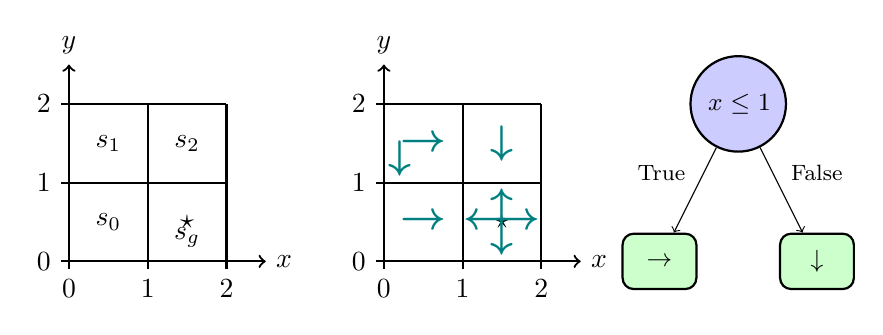
\begin{tikzpicture}[
        decision/.style={circle, draw, thick, fill=blue!20, text width=2.5em, text centered, minimum height=2.5em, font=\small},
        leaf/.style={rectangle, draw, thick, fill=green!20, text width=2em, text centered, rounded corners, minimum height=2em, font=\small},
        edge_label/.style={font=\footnotesize, midway}
    ]
        \tikzstyle{grid}=[draw, thick, fill=gray!10]
        
        % Draw grid
        \draw[grid] (0,0) grid (2,2);
        
        % Add axes
        \draw[thick, ->] (0,0) -- (2.5,0) node[right] {$x$};
        \draw[thick, ->] (0,0) -- (0,2.5) node[above] {$y$};
        
        % Add tick marks and labels
        \foreach \x in {0,1,2} {
            \draw[thick] (\x,0) -- (\x,-0.1) node[below] {$\x$};
        }
        \foreach \y in {0,1,2} {
            \draw[thick] (0,\y) -- (-0.1,\y) node[left] {$\y$};
        }
        
        % Add state labels clockwise from bottom left
        \node at (0.5,0.5) {$s_0$};
        \node at (1.5,0.5) {$\star$};
        \node at (1.5,0.3) {$s_g$};
        \node at (1.5,1.5) {$s_2$};
        \node at (0.5,1.5) {$s_1$};

        % Draid
        \draw[grid] (4,0) grid (6,2);
    
        % Adds
        \draw[thick, ->] (4,0) -- (6.5,0) node[right] {$x$};
        \draw[thick, ->] (4,0) -- (4,2.5) node[above] {$y$};
    
        % Addk marks and labels
        \draw[thick] (4,0) -- (4,-0.1) node[below] {$0$};
        \draw[thick] (5,0) -- (5,-0.1) node[below] {$1$};
        \draw[thick] (6,0) -- (6,-0.1) node[below] {$2$};
    

        \foreach \y in {0,1,2} {
            \draw[thick] (4,\y) -- (3.9,\y) node[left] {$\y$};
        }
        
        % Add state labels clockwise from bottom left
        \node at (4.5,0.5) {\Large{\color{teal} $\boldsymbol{\rightarrow}$}};
        \node at (5.5,0.5) {$\star$};
        \node at (5.5,0.7) {\Large{\color{teal} $\boldsymbol{\uparrow}$}};
        \node at (5.5,0.3) {\Large{\color{teal} $\boldsymbol{\downarrow}$}};
        \node at (5.7,0.5) {\Large{\color{teal} $\boldsymbol{\rightarrow}$}};
        \node at (5.3,0.5) {\Large{\color{teal} $\boldsymbol{\leftarrow}$}};
        \node at (5.5,1.5) {\Large{\color{teal} $\boldsymbol{\downarrow}$}};
        \node at (4.2,1.3) {\Large{\color{teal} $\boldsymbol{\downarrow}$}};
        \node at (4.5,1.5) {\Large{\color{teal} $\boldsymbol{\rightarrow}$}};
        
        \node[decision] (tree5_root) at (8.5,2) {$x \leq 1$};
        \node[leaf] (tree5_right) at (7.5,0) {$\rightarrow$};
        \node[leaf] (tree5_left) at (9.5,0) {$\downarrow$};
        \draw[->] (tree5_root) -- (tree5_right) node[edge_label, above left] {True};
        \draw[->] (tree5_root) -- (tree5_left) node[edge_label, above right] {False};
        \tikzstyle{grid}=[draw, thick, fill=gray!10]
        \end{tikzpicture}}
        \caption{{\small MDP, optimal actions, and an optimal decision tree policy}}\label{fig:mdp-dt}
    \end{subfigure}
    \hfill
    \begin{subfigure}[b]{0.49\textwidth}
        \centering
        \scalebox{0.7}{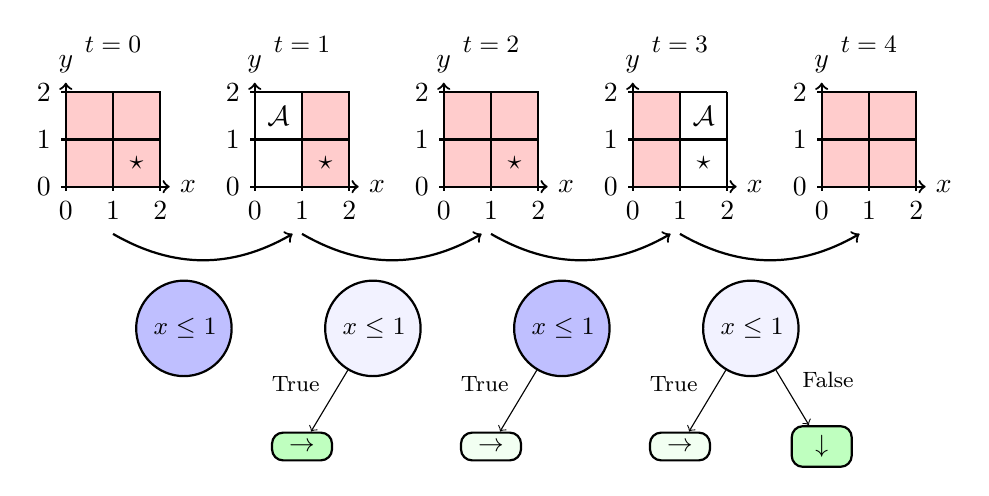
\begin{tikzpicture}[scale=0.6]
    % Define styles
    \tikzstyle{grid}=[draw, thick, fill=gray!10]
    \tikzstyle{rectangle}=[draw, thick, fill=red!20]
    
    % Row 1: IBMDP States (s, o)
    % t=0: Initial state
    \node at (2,7) {\small $t=0$};

    \draw[rectangle] (1,4) rectangle (3,6);
    \draw[grid] (1,4) grid (3,6);
    % Add axes
    \draw[thick, ->] (1,4) -- (3.2,4) node[right] {$x$};
    \draw[thick, ->] (1,4) -- (1,6.2) node[above] {$y$};
    \foreach \x in {0,1,2} {
        \draw[thick] (\x+1,4) -- (\x+1,3.9) node[below] {$\x$};
    }
    \foreach \y in {0,1,2} {
        \draw[thick] (1,\y+4) -- (0.9,\y+4) node[left] {$\y$};
    }
    \node at (2.5, 4.5) {$\star$};
    % \node at (1.5, 5.5) {$\mathcal{A}$};
    
    % Curved arrow from t=0 to t=1
    \draw[thick, ->] (2,3) to[bend right=30] node[midway, below] {} (5.8,3);

    % % t=1: After AIG x≤0.5
    \node at (6,7) {\small $t=1$};

    \draw[rectangle] (6,4) rectangle (7,6);
    \draw[grid] (5,4) grid (7,6);
    % Add axes
    \draw[thick, ->] (5,4) -- (7.2,4) node[right] {$x$};
    \draw[thick, ->] (5,4) -- (5,6.2) node[above] {$y$};
    \foreach \x in {0,1,2} {
        \draw[thick] (\x+5,4) -- (\x+5,3.9) node[below] {$\x$};
    }
    \foreach \y in {0,1,2} {
        \draw[thick] (5,\y+4) -- (4.9,\y+4) node[left] {$\y$};
    }
    \node at (6.5, 4.5) {$\star$};
    \node at (5.5, 5.5) {$\mathcal{A}$};



    % Curved arrow from t=1 to t=2
    \draw[thick, ->] (6,3) to[bend right=30] node[midway, below] {}(9.8,3);

    \node at (10,7) {\small $t=2$};
    
    \draw[rectangle] (9,4) rectangle (11,6);
    \draw[grid] (9,4) grid (11,6);
    % Add axes
    \draw[thick, ->] (9,4) -- (11.2,4) node[right] {$x$};
    \draw[thick, ->] (9,4) -- (9,6.2) node[above] {$y$};
    \foreach \x in {0,1,2} {
        \draw[thick] (\x+9,4) -- (\x+9,3.9) node[below] {$\x$};
    }
    \foreach \y in {0,1,2} {
        \draw[thick] (9,\y+4) -- (8.9,\y+4) node[left] {$\y$};
    }
    \node at (10.5, 4.5) {$\star$};
    % \node at (12.5, 5.5) {$\mathcal{A}$};

    
    % Curved arrow from t=2 to t=4
    \draw[thick, ->] (10,3) to[bend right=30] node[midway, below] {} (13.8,3);
    
    \node at (14,7) {\small $t=3$};

    \draw[rectangle] (13,4) rectangle (14,6);
    \draw[grid] (13,4) grid (15,6);
    % Add axes
    \draw[thick, ->] (13,4) -- (15.2,4) node[right] {$x$};
    \draw[thick, ->] (13,4) -- (13,6.2) node[above] {$y$};
    \foreach \x in {0,1,2} {
        \draw[thick] (\x+13,4) -- (\x+13,3.9) node[below] {$\x$};
    }
    \foreach \y in {0,1,2} {
        \draw[thick] (13,\y+4) -- (12.9,\y+4) node[left] {$\y$};
    }
    \node at (14.5, 4.5) {$\star$};
    \node at (14.5, 5.5) {$\mathcal{A}$};

    
    \draw[thick, ->] (14,3) to[bend right=30] node[midway, below] {} (17.8,3);
    
    % % \node[circle, draw, thick, fill=blue!25, text width=2em, text centered, minimum height=1.5em, font=\small] (tree4_root) at (14.5,0) {$x \leq 1$};
    % % \node[rectangle, draw, thick, fill=green!5, text width=1.5em, text centered, rounded corners, minimum height=1em, font=\small] (tree4_right) at (13,-3) {$\rightarrow$};
    % % \node[rectangle, draw, thick, fill=green!5, text width=1.5em, text centered, rounded corners, minimum height=1em, font=\small] (tree4_left) at (16,-3) {$\downarrow$};
    % % \draw[->] (tree4_root) -- (tree4_right) node[font=\footnotesize, midway, above left] {True};
    % % \draw[->] (tree4_root) -- (tree4_left) node[font=\footnotesize, midway, above right] {False};


    \node at (18,7) {\small $t=4$};
 
    \draw[rectangle] (17,4) rectangle (19,6);
    \draw[grid] (17,4) grid (19,6);
    % % Add axes
    \draw[thick, ->] (17,4) -- (19.2,4) node[right] {$x$};
    \draw[thick, ->] (17,4) -- (17,6.2) node[above] {$y$};
    \foreach \x in {0,1,2} {
        \draw[thick] (\x+17,4) -- (\x+17,3.9) node[below] {$\x$};
    }
    \foreach \y in {0,1,2} {
        \draw[thick] (17,\y+4) -- (16.9,\y+4) node[left] {$\y$};
    }
    % \node at (18.5, 4.5) {$\star$};
    % \node at (18.6, 4.6) {$\mathcal{A}$};


    % \node[circle, draw, thick, fill=blue!5, text width=2em, text centered, minimum height=1.5em, font=\small] (tree4_root) at (19.5,0) {$x \leq 1$};
    % \node[rectangle, draw, thick, fill=green!5, text width=1.5em, text centered, rounded corners, minimum height=1em, font=\small] (tree4_right) at (18,-3) {$\rightarrow$};
    % \node[rectangle, draw, thick, fill=green!25, text width=1.5em, text centered, rounded corners, minimum height=1em, font=\small] (tree4_left) at (21,-3) {$\downarrow$};
    % \draw[->] (tree4_root) -- (tree4_right) node[font=\footnotesize, midway, above left] {True};
    % \draw[->] (tree4_root) -- (tree4_left) node[font=\footnotesize, midway, above right] {False};
    \node[circle, draw, thick, fill=blue!5, text width=2.5em, text centered, minimum height=2.5em, font=\small] (tree4_root) at (15.5,1) {$x \leq 1$};
    \node[rectangle, draw, thick, fill=green!5, text width=1.5em, text centered, rounded corners, minimum height=1em, font=\small] (tree4_right) at (14,-1.5) {$\rightarrow$};
    \node[rectangle, draw, thick, fill=green!25, text width=1.5em, text centered, rounded corners, minimum height=1em, font=\small] (tree4_left) at (17,-1.5) {$\downarrow$};
    \draw[->] (tree4_root) -- (tree4_right) node[font=\footnotesize, midway, above left] {True};
    \draw[->] (tree4_root) -- (tree4_left) node[font=\footnotesize, midway, above right] {False};

    % \node[circle, draw, thick, fill=blue!25, text width=2em, text centered, minimum height=1.5em, font=\small] (tree4_root) at (26.5,5) {$x \leq 1$};
    % \node[rectangle, draw, thick, fill=green!25, text width=1.5em, text centered, rounded corners, minimum height=1em, font=\small] (tree4_right) at (25,2) {$\rightarrow$};
    % \node[rectangle, draw, thick, fill=green!25, text width=1.5em, text centered, rounded corners, minimum height=1em, font=\small] (tree4_left) at (28,2) {$\downarrow$};
    % \draw[->] (tree4_root) -- (tree4_right) node[font=\footnotesize, midway, above left] {True};
    % \draw[->] (tree4_root) -- (tree4_left) node[font=\footnotesize, midway, above right] {False};


    \node[circle, draw, thick, fill=blue!25, text width=2.5em, text centered, minimum height=2.5em, font=\small] (tree4_root) at (11.5,1) {$x \leq 1$};
    \node[rectangle, draw, thick, fill=green!5, text width=1.5em, text centered, rounded corners, minimum height=1em, font=\small] (tree4_right) at (10,-1.5) {$\rightarrow$};
    % \node<6->[rectangle, draw, thick, fill=green!5, text width=1.5em, text centered, rounded corners, minimum height=1em, font=\small] (tree4_left) at (16,-3) {$\downarrow$};
    \draw[->] (tree4_root) -- (tree4_right) node[font=\footnotesize, midway, above left] {True};
    % \draw<6->[->] (tree4_root) -- (tree4_left) node[font=\footnotesize, midway, above right] {False};

    \node[circle, draw, thick, fill=blue!5, text width=2.5em, text centered, minimum height=2.5em, font=\small] (tree4_root) at (7.5,1) {$x \leq 1$};
    \node[rectangle, draw, thick, fill=green!25, text width=1.5em, text centered, rounded corners, minimum height=1em, font=\small] (tree4_right) at (6,-1.5) {$\rightarrow$};
    \draw[->] (tree4_root) -- (tree4_right) node[font=\footnotesize, midway, above left] {True};

    \node[circle, draw, thick, fill=blue!25, text width=2.5em, text centered, minimum height=2.5em, font=\small] (tree4_root) at (3.5,1) {$x \leq 1$};
    % \node<5>[rectangle, draw, thick, fill=green!5, text width=1.5em, text centered, rounded corners, minimum height=1em, font=\small] (tree4_right) at (3,-3) {$\rightarrow$};
    % \node<5>[rectangle, draw, thick, fill=green!5, text width=1.5em, text centered, rounded corners, minimum height=1em, font=\small] (tree4_left) at (6,-3) {$\downarrow$};
    % \draw<5>[->] (tree4_root) -- (tree4_right) node[font=\footnotesize, midway, above left] {True};
    % \draw<5>[->] (tree4_root) -- (tree4_left) node[font=\footnotesize, midway, above right] {False};

    
\end{tikzpicture}}
        \caption{{\small An associated IBMDP trajectory.}}\label{fig:ibmdp-example}
    \end{subfigure}
    \caption{Figure~\ref{fig:mdp-dt} shows a four-state grid world MDP with four directional actions and zero reward except at the goal state ($\star$). The center illustrates an optimal policy, and the right an optimal depth-1 decision tree that tests state coordinates to choose actions. Figure~\ref{fig:ibmdp-example} depicts an IBMDP trajectory for this grid world. Observations $\boldsymbol{o}_t$ encode bounds on the agent’s unknown state features: initially $\boldsymbol{o}_0=(0,2,0,2)$ (“the state could be anywhere”). Information-gathering actions iteratively refine these bounds, corresponding to internal tree tests. For example, at $t=0$ the IGA $\langle x,1\rangle$ yields reward $\zeta$ and updates the observation to $\boldsymbol{o}_1=(0,1,0,2)$. A downstream action then moves the agent, gives reward 0, resets the bounds, and the process repeats until reaching the absorbing goal state. Masking the true state forces the agent to gather information to act optimally.}
\end{figure*}

\subsection{Markov decision processes}

Markov decision processes were first introduced in the 1950s by Richard Bellman~\cite{Bellman}.
Informally, an MDP models how an agent acts over time to achieve a goal. 
At every time step, the agent observes its current state (e.g., patient weight and tumor size) and takes an action (e.g., administers a certain amount of chemotherapy).
The agent receives a reward that helps evaluate the quality of the action with respect to the goal (e.g., tumor size decrease when the objective is to cure cancer).
Finally, the agent transitions to a new state (e.g., the updated patient state) and repeats this process over time:
\begin{definition}[Markov decision process]\label{def:mdp} An MDP is a tuple $\mathcal{M} = \langle S, A, R, T, T_0 \rangle$.
$S$ is a finite set of states representing all possible configurations of the environment.
$A$ is a finite set of actions available to the agent.
$R: S \times A \rightarrow \mathbb{R}$ is a deterministic reward function that assigns a real-valued reward to each state-action pair. While in general reward functions are often stochastic, in this manuscript we focus deterministic ones without loss of generality.
$T: S \times A \rightarrow \Delta(S)$ is the transition function that maps state-action pairs to probability distributions over next states $\Delta(S)$.
$T_0 \in \Delta(S)$ is the initial distribution over states.
\end{definition}

Informally, we would like to act in an MDP so that we obtain as much reward as possible over time.
We can formally define this objective, that we call the reinforcement learning objective, as follows:

\begin{definition}[Reinforcement learning objective]\label{def:mdp-obj} Given an MDP (definition~\ref{def:mdp}) $\mathcal{M}\equiv\langle S, A, R, T, T_0 \rangle$, the goal of reinforcement learning for sequential decision making is to find a model, also known as a policy, $\pi: S \rightarrow A$ that maximizes the expected discounted sum of rewards:
{\small
$$J(\pi) = \mathbb{E}\left[\sum_{t=0}^{\infty} \gamma^t R(s_t, \pi(s_t)) \mid s_0 \sim T_0, s_{t+1} \sim T(s_t, \pi(s_t))\right]$$}
where $0< \gamma\leq 1$ is the discount factor that controls the trade-off between immediate and future rewards.
\end{definition}

Algorithms presented in this article aim to find an optimal policy $\pi^\star \in\underset{\pi}{\operatorname{argmax}}\ J(\pi)$ that maximizes the above reinforcement learning objective.
In particular, RL algorithms~\cite{sutton,pg_sutton,watkins1992q,dqn,ppo} learn such optimal policies using data of MDP interactions without prior knowledge of the reward and transition models.
Useful quantities for such algorithms include \textit{value} of states and actions.
\begin{definition}[Value of a state]\label{def:vs} 
    In an MDP $\mathcal{M}$ (definition~\ref{def:mdp}), the value of a state $s\in S$ under policy $\pi$ is the expected discounted sum of rewards starting from state $s$ and following policy $\pi$:
    {\small
    $$V^\pi(s) = \mathbb{E}\left[\sum_{t=0}^{\infty} \gamma^t R(s_t, \pi(s_t)) \mid s_0 = s, s_{t+1} \sim T(s_t, \pi(s_t))\right]$$}
    Applying the Markov property gives a recursive definition of the value of $s$ under policy $\pi$: $V^\pi(s) = R(s,\pi(s)) + \gamma \mathbb{E}\left[V^\pi(s') | s'\sim T(s, \pi(s))\right]$.
    The optimal value of a state $s\in S$, $V^\star(s)$, is the value of state $s$ when following the optimal policy $\pi^{\star}$ (the policy that maximizes the RL objective (definition~\ref{def:mdp-obj})): $V^{\star}(s) = V^{\pi^{\star}}(s)$.
    Similarly, the optimal value of a state–action pair $(s,a)\in S\times A$, $Q^\star(s,a)$, is the value when taking action $a$ in state $s$ and then following the optimal policy: $Q^{\star}(s,a) = R(s, a) + \gamma\mathbb{E}\left[V^{\star}(s') | s'\sim T(s, a)\right]$.
\end{definition}

\subsection{Decision tree policies}
While other interpretable policy classes exist~\cite{kohler2025evaluating}, one conjecture from~\citet{glanois-survey} is that interpretable models are all hard to optimize or learn because they are non-differentiable in nature.
This is something that will be key in our study of decision tree policy that we introduce next.

\begin{definition}[Decision tree policy]\label{def:dt}
    A decision tree policy is a rooted tree $\pi_{\mathcal{T}} = (\mathcal{N}, E)$.
    Each internal node $\nu \in \mathcal{N}$ is associated with a test that maps an MDP state attribute to a Boolean, e.g. $s_{i}\leq v$ for $v\in \mathbb{R}$.
    Each edge $e \in E$ from an internal node corresponds to an outcome of the associated test function.
    Each leaf node $l \in \mathcal{N}$ is associated with an MDP action $a_l \in A$.
    For any input $s \in S$, the tree defines a unique path from root to leaf, determining the prediction $\pi_{\mathcal{T}}(s) = a_l$ where $l$ is the reached leaf.
    The depth of a tree is the maximum path length from root to any leaf.
\end{definition}

In figure~\ref{fig:mdp-dt}, we present an example Markov decision process (definition~\ref{def:mdp}), the optimal actions that maximize the RL objective (definition~\ref{def:mdp-obj}), and a decision tree policy (definition~\ref{def:dt}) that also maximizes the RL objective.
Next, we present the class of MDPs introduced in~\citet{topin2021iterative} useful for our to understand reinforcement learning of decision tree policies that directly optimize the RL objective in an MDP.

\subsection{Iterative bounding Markov decision processes}\label{sec:ibmdp}
Iterative bounding MDPs (IBMDPs) are, as the name suggests, standard MDPs (definition~\ref{def:mdp}) and therefore admit optimal deterministic Markovian policies~\cite{Bellman}. We assume continuous state spaces with finite action sets, using bold notation for vector-valued states and observations (though our results also extend to discrete states).

Given a downstream MDP where we seek a decision tree policy, an IBMDP augments the state with additional observations that iteratively refine knowledge about the downstream state features. Actions include (i) downstream actions that affect the environment and receive the same rewards as in the original MDP, and (ii) information-gathering actions (IGAs) that update the observations. IGAs receive a chosen reward so that optimizing the IBMDP objective captures a trade-off between downstream performance and interpretability.

We now formally define IBMDPs following~\citet{topin2021iterative}.
\begin{definition}[Iterative bounding Markov decision process (\citet{topin2021iterative}, section 4.1)]\label{def:ibmdp}
Given a downstream MDP $\mathcal{M}\equiv\langle S, A, R, T, T_0 \rangle$ (definition~\ref{def:mdp}), an associated iterative bounding Markov decision process $\mathcal{M}_{IB}$ is a tuple:
\begin{align*}
    \langle \overbrace{S \times O}^{\text{State space}}, \overbrace{A \cup A_{info}}^{\text{Action space}}, \overbrace{(R, \zeta)}^{\text{Reward}}, \overbrace{(T_{info}, T, T_0)}^{\text{Transitions}}\rangle
\end{align*}
$S$ are the downstream MDP state features. Downstream state features $\boldsymbol{s} = (s_1, \dots, s_p)\in S$ are bounded: $s_j \in [L_j, U_j]$ where $\infty < L_j \leq U_j < \infty \ \forall 1\leq j \leq p$.
$O$ are observations. They represent bounds on the downstream state features: $O\subsetneq S^2 =  [L_1, U_1]\times \dots \times [L_p, U_p] \times [L_1, U_1]\times \dots \times [L_p, U_p]$. So the complete IBMDP state space is $S \times O$: the concatenations of downstream state features and observations.
Given some downstream state features $\boldsymbol{s} = (s_1, \dots, s_p)\in S$ and some observation $\boldsymbol{o} = (L_1, U_1, \dots, L_p, U_p)$, an IBMDP state is $\boldsymbol{s}_{IB} = (\overbrace{s_1, \dots, s_p}^{\text{downstream state features}}, \overbrace{L_1, U_1, \dots, L_p, U_p}^{\text{observation}})$.
$A$ are the downstream MDP actions.
$A_{info}$ are \textit{information-gathering} actions of the form $\langle j, v \rangle$ where $j$ is a state feature index $1 \leq j \leq p$ and $v$ is a real number between $L_j$ and $U_j$. So the complete action space of an IBMDP is the set of downstream MDP actions and information-gathering actions $A \cup A_{info}$.
$R: S\times A \rightarrow \mathbb{R}$ is the downstream MDP reward function.
$\zeta$ is a reward signal for taking an information-gathering action.
So the IBMDP reward function is to get a reward from the downstream MDP if the action is a downstream MDP action or to get $\zeta$ if the action is an IGA action.
$T_{info}: S\times O \times( A_{info} \cup A )\rightarrow \Delta (S\times O)$ is the transition function of IBMDPs: 
given some observation $\boldsymbol{o}_t = (L'_1, U'_1, \dots, L'_p, U'_p) \in O$ and downstream state features $\boldsymbol{s}_t=(s'_1, s'_2, \dots, s'_p)$ if an IGA $\langle j, v \rangle$ is taken, the new observation $\boldsymbol{o}_{t+1}$ is $(L'_1, U'_1, \dots , L'_j, \min\{v, U'_j\}, \dots , L'_p, U'_p) \text{ if } s_j \leq v$ or $(L'_1, U'_1, \dots , \max\{v, L'_j\}, U'_j, \dots , L'_p, U'_p) \text{ if } s_j > v$.
If a downstream action is taken, the observation is reset to the default downstream state feature bounds $(L_1, U_1,\dots, L_p, U_p)$ and the downstream state features change according to the downstream MDP transition function: $\boldsymbol{s}_{t+1}\sim T(\boldsymbol{s}_t, a_t)$.
At initialization, the downstream state features are drawn from the downstream MDP initial distribution $T_0$ and the observation is always set to the default downstream state features bounds $\boldsymbol{o}_0=(L_1, U_1,\dots, L_p, U_p)$.
\end{definition}

We present an IBMDP for a the grid-world MDP (figure~\ref{fig:mdp-dt}) in figure~\ref{fig:ibmdp-example}.
Now remains to extract a decision tree policy (definition~\ref{def:dt}) for a downstream MDP $\mathcal{M}$ from a policy for an associated IBMDP $\mathcal{M}_{IB}$. 

\subsection{From policies to trees}
information-gathering actions (definition~\ref{def:ibmdp}) resemble the tests $1_{\{x_{\_, j} \leq v\}}$ that make up internal decision tree nodes (figure~\ref{fig:ibmdp-example}).
Indeed, a policy taking actions in an IBMDP essentially builds a tree by taking sequences of IGAs (internal nodes) and then a downstream action (leaf node) and repeats this process over time.
In particular, the IGA rewards $\zeta$ can be seen as a regularization or a penalty for interpretability: if $\zeta$ is very small compared to downstream rewards, a policy will try to take downstream actions as often as possible, i.e. build shallow trees with short paths between root and leaves.

\citet{topin2021iterative} show that only a subset of IBMDP policies correspond to downstream decision tree policies. Their extraction algorithm (algorithm~\ref{alg:extract-tree}) requires deterministic policies that depend only on IBMDP observations. Non-deterministic policies would yield stochastic decision trees~\cite{stoch-decision}, whose interpretability remains unclear. Policies that depend on the full IBMDP state also defeat the purpose of information-gathering actions, since the agent already has all necessary state information to act optimally.
The connections between partially observable MDPs (POMDPs~\cite{POMDP,chap2}) and extracting decision tree policies from IBMDPs might seem obvious but they are absent from the original IBMDP paper~\cite{topin2021iterative} and from subsequent work.
In the next section we bridge this gap.
\section{Bridging the gap with the partially observable MDPs literature}\label{sec:poibmdp}
\subsection{An adequate formalism}
To better understand reinforcement learning of decision tree policies for MDPs, we explictly re-write the problem of optimizing a deterministic policy depending on current observations in an IBMDP as the problem of optimizing a deterministic policy depending only on current observations--also known as a deterministic \emph{memoryless} policy--in a partially observable Markov decision process (POMDP~\cite{POMDP}).
By doing so, we can leverage results from the POMDP literature that is richer than interpretable reinforcement learning literature.

\begin{definition}[Partially observable Markov decision process]\label{def:pomdp}
A partially observable Markov decision process is a tuple $\langle X, A, O, R, T, T_0, \Omega\rangle$. $X$ is the hidden state space.
$A$ is a finite set of actions.
$O$ is a set of observations.
$T: X \times A \rightarrow \Delta(X)$ is the transition function, where $T(\boldsymbol{x}_t, a, \boldsymbol{x}_{t+1}) = P(\boldsymbol{x}_t|\boldsymbol{x}_{t+1}, a)$ is the probability of transitioning to state $\boldsymbol{x}_{t}$ when taking action $a$ in state $\boldsymbol{x}$.
$T_0$: is the initial distribution over states. 
$\Omega: X \rightarrow \Delta(O)$ is the observation function, where $\Omega(\boldsymbol{o}, a, \boldsymbol{x}) = P(\boldsymbol{o}|\boldsymbol{x}, a)$ is the probability of observing $\boldsymbol{o}$ in state $\boldsymbol{x}$.
$R: X \times A \rightarrow \mathbb{R}$ is the reward function, where $R(\boldsymbol{x}, a)$ is the immediate reward for taking action $a$ in state $\boldsymbol{x}$.
Note that $\langle X, A, R, T, T_0 \rangle$ defines an MDP (definition~\ref{def:mdp}).
\end{definition}

Next, we can define partially observable iterative bounding Markov decision processes (POIBMDPs). 
They are IBMDPs (definition~\ref{def:ibmdp}) for which we explicitly define an observation space and an observation function.

\begin{definition}[Partially observable iterative bounding Markov decision process]\label{def:poibmdp} a partially observable iterative bounding Markov decision process $\mathcal{M}_{POIB}$ is a tuple:
    \begin{align*}
        \langle \overbrace{S\times O}^{\text{States}}, \overbrace{A\cup A_{info}}^{\text{Action space}},\overbrace{O}^{\text{Observations}} ,\overbrace{(R, \zeta)}^{\text{Rewards}}, \overbrace{(T_{info}, T, T_0)}^{\text{Transitions}}, \Omega \rangle
    \end{align*}
    , where $\langle S\times O, A\cup A_{info}, (R, \zeta),( T, T_0, T_{info})\rangle$ is an IBMDP (definition~\ref{def:ibmdp}).
    The transition function $\Omega$ maps concatenation of state features and observations--IBMDP states--to observations, $\Omega:S\times O \rightarrow O$, with $P(\boldsymbol{o}|(\boldsymbol{s}, \boldsymbol{o}))=1$ 
\end{definition}
POIBMDPs are particular instances of POMDPs where the observation function simply applies a mask over some features of the hidden state.
This setting has other names in the literature.
For example, POIBMDPs are mixed observability MDPs \cite{momdp} with downstream MDP state features as the \textit{hidden variables} and feature bounds as \textit{visible} variables.
POIBMDPs can also be seen as non-stationary MDPs (N-MDPs)~\cite{learning-pomdp} in which there is one different transition function per downstream MDP state: these are called hidden-mode MDPs~\cite{hmmdp}.
Following~\cite{learning-pomdp} we can write the value of a deterministic memoryless policy $\pi:O\rightarrow A\cup A_{info}$ in observation $\boldsymbol{o}$.

\begin{definition}[Value of an observation]\label{def:vpo} In a POIBMDP (definition~\ref{def:poibmdp}), the expected cumulative discounted reward of a deterministic memoryless policy $\pi:O\rightarrow A\cup A_{info}$ starting from observation $o$ is $V^{\pi}(\boldsymbol{o})$:
$V^{\pi}(\boldsymbol{o}) &= \underset{(s,\boldsymbol{o}')\in S\times O}{\sum}P^{\pi}((\boldsymbol{s}, \boldsymbol{o}')|\boldsymbol{o})V^{\pi}((\boldsymbol{s}, \boldsymbol{o}'))$.
With $P^{\pi}((\boldsymbol{s}, \boldsymbol{o}')|\boldsymbol{o})$ the asymptotic occupancy distribution (see section 4 from~\citet{learning-pomdp} for the full definition) of the hidden POIBMDP state $(\boldsymbol{s},\boldsymbol{o}')$ given the partial observation $o$ and $V^{\pi}((s, o'))$ the classical state-value function (definition~\ref{def:vs}).
We abuse notation and denote both values of observations and values of states by $V$ since the function input is not ambiguous.
\end{definition}

\subsection{Reinforcement learning in POMDP}\label{sec:asym}

In general, the policy that maximizes the RL objective (definition~\ref{def:mdp-obj}) in a POMDP (definition~\ref{def:pomdp}) maps ``belief states'' or observation histories to actions~\cite{chap2}.
Hence, those policies do not correspond to decicion trees since we require that policies depend only on the current observation (algorithm~\ref{alg:extract-tree}).
If we did not have this constraint, we could apply any standard RL algorithm to solve POIBMDPs by seeking policies depending on belief states or observations histories because those are sufficient to optimally control any POMDP~\cite{chap2,lambrechts2025informed}.

In particular, the problem of finding the optimal deterministic memoryless policies for POMDPs is NP-HARD, even with full knowledge of transitions and rewards(section3.2 from~\citet{littman1}).
It means that it is impractical to enumerate all possible policies and take the best one. 
For even moderate-sized POMDPs, a brute-force approach would take a very long time since there are $|A|^{|O|}$ deterministic memoryless policies.
Hence it is interesting to study reinforcement learning for finding the best deterministic memoryless policy since it would not enumerate the whole solution space.

In~\citet{learning-pomdp}, the authors show that the optimal memoryless policy can be stochastic. Hence, policy gradient algorithms~\cite{pg_sutton}--that return stochastic policies--are to avoid since we seek the best \textit{deterministic} policy. 
Furthermore, the optimal deterministic memoryless policy might not maximize all the values of all observations simultaneously~\cite{learning-pomdp} which makes it difficult to use TD-learning algorithms like Q-learning~\cite{watkins1992q}.
Indeed, doing a TD-learning update of one observation's value (definition~\ref{def:vpo}) can change the value of \textit{all} other observations in an uncontrollable manner because of the dependence in $P^{\pi}((s, \boldsymbol{o}')|\boldsymbol{o})$ (definition~\ref{def:vpo}).

Despite theoretical hardness, simple RL methods that treat observations as states (e.g., Q-learning or Sarsa~\cite{sutton}) often work well in POMDPs~\cite{sarsa-pomdp}. More recently, asymmetric RL~\cite{baisero-dqn,baisero-ppo} has shown promise by training both a hidden-state model (available only during training) and an observation- or history-based model for deployment.
In appendix~\ref{sec:hp-pomdp}, we present tabular asymmetric RL methods such as asymmetric Q-learning, which learns an observable Q-function $Q:O\times A\to\mathbb{R}$ using a hidden-state target $U:X\times A\to\mathbb{R}$. This matches the modified DQN approach of~\citet{topin2021iterative}, and we provide a reproducibility study in appendix~\ref{sec:reprod}.

While asymmetric RL was long supported mainly by empirical results,~\citet{justif-asym} recently proved it can theoretically improve history-dependent or memoryless policies in POMDPs. However, these methods are currently impractical, as they require costly Monte Carlo estimates of occupancy distributions. We leave their practical integration to future work.
\section{Methodology}\label{sec:methodology}
The goal of this section is to check if the aforementioned approach can consistently retrieve optimal decision tree policies for a simple grid world MDP (figure~\ref{fig:mdp-dt}).
In particular, we use reinforcement learning to train decision tree policies for MDPs by seeking deterministic memoryless policies that optimize the RL objective in POIBMDPs (figure~\ref{fig:ibmdp-example} and section~\ref{sec:poibmdp}).

\subsection{Computing some decision tree policies}
To assess the performance of reinforcement learning, for different trade-off reward $\zeta$ (definition~\ref{def:ibmdp}), we identify the deterministic memoryless policies that maximize the RL objective (definition~\ref{def:mdp-obj}). Each of those policies correspond to one of the decision tree policies for the grid world downstream MDP illustrated in figure~\ref{fig:irl-objectives}: (i) a depth-0 tree equivalent to always taking the same downstream action ($\pi_{\mathcal{T}_0}$), (ii) a depth-1 tree equivalent alternating between an IGA and a downstream action ($\pi_{\mathcal{T}_1}$), (iii) an unbalanced depth-2 tree that sometimes takes two IGAs then a downstream action and sometimes a an IGA then a downstream action ($\pi_{\mathcal{T}_u}$), (iv) a depth-2 tree that alternates between taking two IGAs and a downstream action ($\pi_{\mathcal{T}_2}$), or (v) an infinite `tree'' that only takes IGAs. We will particularly focus on trying to retrieve the depth-1 decision tree that is the most interpretable--smallest number of nodes and shallowest--tree taking optimal actions. Because from~\citet{learning-pomdp} we know that for POMDPs, stochastic memoryless policies can sometimes get better expected discounted rewards than deterministic memoryless policies, we also compute the value of the stochastic policy that randomly alternates between two downstream actions: $\rightarrow$ and $\downarrow$. Taking those two downstream actions always lead to the goal state in expectation (figure~\ref{fig:mdp-dt}). Because we know all the downstream states, all the observations, all the actions, all the rewards and all the transitions of our POIBMDPs, we can compute the RL objective values of those different deterministic memoryless policies exactly given $\zeta$ and $\gamma$ a discount factor. We plot, in figure~\ref{fig:irl-objectives}, the RL objective values of the decision tree policies as functions of $\zeta$ when we fix $\gamma=0.99$ (standard choice of discount in practice~\cite{sutton}). Despite objective values being very similar for the depth-1 and unbalanced depth-2 tree, we now know from the green shaded area that a depth-1 tree is optimal when $0< \zeta < 1$ in the POIBMDP. 
Interestingly, two challenges of learning in POMDPs described in~\cite{learning-pomdp} are visible in figure~\ref{fig:irl-objectives}. First, there is a whole range of $\zeta$ values for which the optimal memoryless policy is stochastic. Second, for e.g. $\zeta=0.5$, while the optimal deterministic memoryless policy corresponds to a depth-1 tree, the value of the (PO)IBMDP state $(\boldsymbol{s}_2, \boldsymbol{o}_0) = (1.5, 1.5, 0, 2, 0, 2)$, i.e. the agent current position is upper right cell in the downstream MDP but it has not information about it, is not maximized by the optimal memoryless policy that will take 1 information-gathering action in between each downstream action (figure~\ref{fig:irl-objectives}), but by the sub-optimal policy that always goes down. Next, we present the specific experimental setup that we use in the remaining of the paper.
\begin{figure*}
    \begin{subfigure}{0.55\textwidth}
    \centering
    \scalebox{0.55}{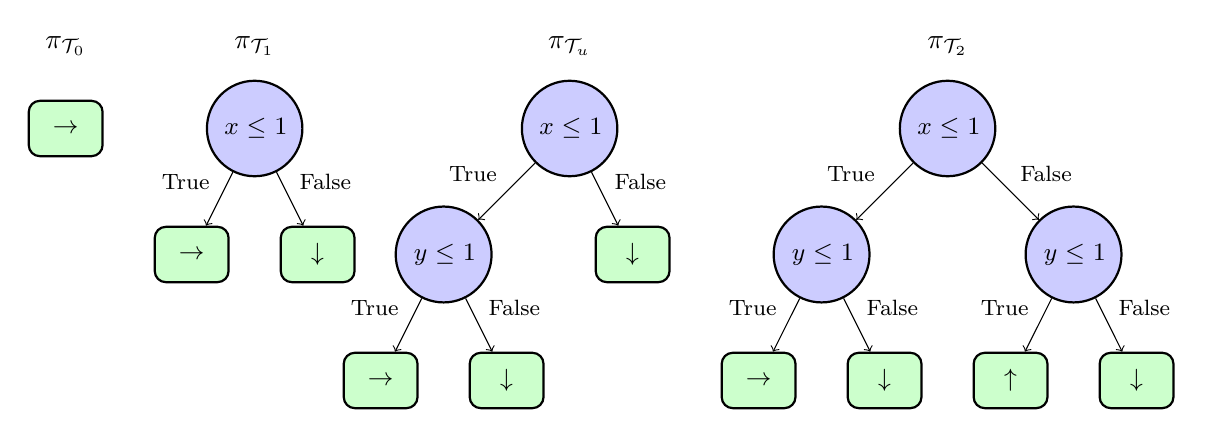
\begin{tikzpicture}[
        scale=0.8,
        decision/.style={circle, draw, thick, fill=blue!20, text width=2.5em, text centered, minimum height=2.5em, font=\small},
        leaf/.style={rectangle, draw, thick, fill=green!20, text width=2em, text centered, rounded corners, minimum height=2em, font=\small},
        edge_label/.style={font=\footnotesize, midway}
    ]
        
        \node[leaf] at (-3, 0) {$\rightarrow$};
        % Tree 4: if x <= 0.5 move right else move left
        \node[decision] (tree4_root) at (0,0) {$x \leq 1$};
        \node[leaf] (tree4_right) at (-1,-2) {$\rightarrow$};
        \node[leaf] (tree4_left) at (1,-2) {$\downarrow$};
        \draw[->] (tree4_root) -- (tree4_right) node[edge_label, above left] {True};
        \draw[->] (tree4_root) -- (tree4_left) node[edge_label, above right] {False};
        
        % Draw a square around the tree
        % \draw[thick, red] (-2, 1.8) rectangle (2, -2.5);

        % Tree 7: if x <= 0.5 and y <= 0.5 move right else move down
        \node[decision] (tree7_root) at (5,0) {$x \leq 1$};
        \node[decision] (tree7_y) at (3,-2) {$y \leq 1$};
        \node[leaf] (tree7_right) at (2,-4) {$\rightarrow$};
        \node[leaf] (tree7_down) at (4,-4) {$\downarrow$};
        \node[leaf] (tree7_down2) at (6,-2) {$\downarrow$};
        \draw[->] (tree7_root) -- (tree7_y) node[edge_label, above left] {True};
        \draw[->] (tree7_root) -- (tree7_down2) node[edge_label, above right] {False};
        \draw[->] (tree7_y) -- (tree7_right) node[edge_label, above left] {True};
        \draw[->] (tree7_y) -- (tree7_down) node[edge_label, above right] {False};


        \node[decision] (tree7_root) at (11,0) {$x \leq 1$};
        \node[decision] (tree7_y) at (9,-2) {$y \leq 1$};
        \node[decision] (tree7_y2) at (13,-2) {$y \leq 1$};
        \node[leaf] (tree7_right) at (8,-4) {$\rightarrow$};
        \node[leaf] (tree7_down) at (10,-4) {$\downarrow$};
        \node[leaf] (tree7_right2) at (12,-4) {$\uparrow$};
        \node[leaf] (tree7_down2) at (14,-4) {$\downarrow$};
        \draw[->] (tree7_root) -- (tree7_y) node[edge_label, above left] {True};
        \draw[->] (tree7_root) -- (tree7_y2) node[edge_label, above right] {False};
        \draw[->] (tree7_y) -- (tree7_right) node[edge_label, above left] {True};
        \draw[->] (tree7_y) -- (tree7_down) node[edge_label, above right] {False};
        \draw[->] (tree7_y2) -- (tree7_right2) node[edge_label, above left] {True};
        \draw[->] (tree7_y2) -- (tree7_down2) node[edge_label, above right] {False};

        % Labels
        \node[above] at (-3,1) {$\pi_{\mathcal{T}_0}$};
        \node[above] at (0,1) {$\pi_{\mathcal{T}_1}$};
        \node[above] at (5,1) {$\pi_{\mathcal{T}_u}$};
        \node[above] at (11,1) {$\pi_{\mathcal{T}_2}$};


    \end{tikzpicture}}
\end{subfigure}
\hfill
\begin{subfigure}{0.45\textwidth}
    \centering
    \includegraphics[width=0.95\textwidth]{../images/images_part1/objective_values_plot.pdf}
\end{subfigure}
\caption{Decision tree policies and their RL objective values (definition~\ref{def:mdp-obj}) as functions of the rewards $\zeta$ in POIBMDPs associated to the grid world MDP (figure~\ref{fig:ibmdp-example}). Shaded areas on the right plot indicate which deterministic memoryless policy is optimal depending on $\zeta$.
Recall that $\zeta$ can be seen as a reward that encourages the deterministic memoryless policy to take information-gathering actions, i.e. the reward that trades off interpretability of the corresponding decision tree and its cumulative reward.}\label{fig:irl-objectives}
\end{figure*}

\subsection{Experimental setup}
All our code is open source\footnote{\url{https://anonymous.4open.science/r/poibmdps-5BFE/}}.
The downstream MDP for which we want to learn decision tree policies with reinforcement learning is the grid world MDP (figure~\ref{fig:mdp-dt}).
We then get 100 associated POIBMDPs following figure~\ref{fig:ibmdp-example} with $\zeta$ chosen uniformly among 100 different in $]0, 1[$. 

We will evaluate two types of reinforcement learning algorithm.
Frist we use standard tabular RL algorithms, namely Q-learning, Sarsa, and vanilla policy gradient on a softmax policy~\cite{watkins1992q,sutton,jsj}, to learn deterministic memoryless policies in POIBMDPs by simply replacing the current state in the algorithm descriptions by the current observation.
In theory the policy gradient algorithm should not be a good candidate for our problem since it searches for stochastic policies that we showed can be better than our sought depth-1 decision tree policy (figure~\ref{fig:irl-objectives}), but for completeness we will see what trees are obtained after greddification of the stochastic policies.

Second, we also use the more specialised asymmetric Q-learning, asymmetric Sarsa, and asymmetric policy gradient (algorithm~\ref{alg:asymqlearning}, section~\ref{sec:asym}).
Each algorithm is trained until convergence on each POIBMDP, and each one of those runs is repeated 100 times.
For all baselines we use, when applicable, exploration rates $\epsilon=0.3$ and learning rates $\alpha=0.1$.
All the training curves are presented in appendix~\ref{sec:training}.

We will consider two metrics.
We consider the distribution of the learned trees over the 100 training seeds.
Indeed, since for every POIBMDP we run each algorithm 100 times, at the end of training we get 100 deterministic memoryless policies, from which we can extract the equivalent 100 decision tree policies using algorithm~\ref{alg:extract-tree} and we can count which one have e.g. a depth of 1.
This helps understand which trees RL algorithms tend to learn as a function of the trade-off reward $\zeta$.


\subsection{Can reinforcement learning find the optimal deterministic memoryless POIBMDP policies?}\label{sec:experiments}

In figure~\ref{fig:dt-distrib-poibmdp}, we plot the distributions of the final learned trees over the 100 random seeds in function of $\zeta$ from the above runs.
For example, in figure~\ref{fig:dt-distrib-poibmdp}, in the top left plot, when learning 100 times in a POIBMDP with $\zeta=0.5$, Q-learning returned almost 100 times a depth-0 tree.
Again, on none of those subplots do we see a high rate of learned depth-1 trees for $\zeta\in ]0, 1[$.
It is alerting that the most frequent learned trees are the depth-0 trees for $\zeta\in ]0, 1[$ because such trees are way more sub-optimal than e.g. the depth-2 unbalanced trees (figure~\ref{fig:irl-objectives}).  
One interpretation of this phenomenon is that the learning in POIBMDPs is very difficult and so agents tend to converge to trivial policies, e.g., repeating the same downstream action.
Furhtermore, in appendix~\ref{sec:training} we show that for POIBMDPs with $\zeta \in [-1, 0]$ and $\zeta \in [1, 2]$, baselines consistently learn the optimal policies--a depth-0 tree and an infinite tree respectively--which is concerning as it means that RL seem to find only trivial policies.
On the positive side, we observe that asymmetric versions of Q-learning and Sarsa have found the optimal deterministic memoryless policy--the depth-1 decision tree--more frequently throughout the optimality range $]0,1[$, than their symmetric counter-parts for $\zeta\in ]0, 1[$.
Next, we quantify how difficult it is to do RL to learn memoryless policies in POIBMDPs as opposed to standard Markovian polciies.

\begin{figure}
    \centering
    \includegraphics[width=0.4\textwidth]{../slides_soutenance/tree_distributions.pdf}
    \caption{Distributions of final tree policies learned across the 100 seeds.
    For each $\zeta$ value, there are four colored points. Each point represent the share of depth-0 trees (red), depth-1 trees (green), unbalanced depth-2 trees (orange) and depth-2 trees (blue).
    }\label{fig:dt-distrib-poibmdp}
\end{figure}


\subsection{How difficult is it to learn in POIBMDPs?}\label{sec:how-diff}

In this section we run the same (asymmetric) reinforcement learning algorithms to learn standard Markovian policies in MDPs (definition~\ref{def:mdp}) or IBMDPs (definition~\ref{def:ibmdp}), or deterministic memoryless policies in POIBMDPs (definition~\ref{def:poibmdp}).

In order to see how difficult each of these three problems is, we can run a \textit{great} number of experiments for each problem and compare solving rates.
To make solving rates comparable we consider a unique instance for each of those problems.
Problem 1 is learning one of the optimal standard Markovian deterministic policy ($\pi: S\rightarrow A$)from figure~\ref{fig:mdp-dt} for the grid world MDP with $\gamma=0.99$.
Problem 2 is learning one of the optimal standard Markovian deterministic policy ($\pi: S\times O \rightarrow A \cup A_{info}$) for the IBMDP from figure~\ref{fig:ibmdp-example} with $\gamma=0.99$ and $\zeta=0.5$.
Problem 3 is what has been done in the previous section to learn deterministic memoryless policies ($\pi: O \rightarrow A \cup A_{info}$) where in addition of fixing $\gamma=0.99$ we also fix $\zeta=0.5$.

We use the six (asymmetric) RL algorithms from the previous section and try a wide set of hyperparameters and additional learning tricks (optimistic Q-function, eligibility traces, entropy regularization and $\epsilon$-decay, all are described in \cite{sutton}).
The complete detailed lists of hyperparameters are given in the appendix~\ref{sec:hp-pomdp} and a summary is given in table~\ref{tab:ib-params}.
Furthermore, the careful reader might notice that there is no point running asymmetric RL on MDPs or IBMDPs when the problem does not require partial observability.
Hence, we only run asymmetric RL for POIBMDPs and otherwise run all other RL algorithms and all problems.

Each unique hyperparameter combination for a given algorithm on a given problem is run 10 times on 1 million learning steps to get standard errors.
For example, for asymmetric Sarsa, we run a total of $10\times 768= 7680$ experiments for learning deterministic memoryless policies for a POIBMDP.
To get a success rate, we can simply divide the number of learned optimal depth-1 tree by 768 (recall that for $\gamma=0.99$ and $\zeta=0.5$, the optimal policy is a depth-1 tree (e.g. figure~\ref{fig:irl-objectives}). 


The key observations from figure~\ref{fig:po-vs-ib} is that reinforcement learning a deterministic memoryless policy in a POIBMDP, is way harder than learning a standard Markovian policy.
For example, Q-learning finds the optimal solution in only 3\% of the experiments while the same algorithms to optimize the standard RL objective (definition~\ref{def:mdp-obj}) in an MDP or IBMDP found the optimal solutions 50\% of the time.
Even though asymmetry seems to increase performances; learning a decision tree policy for a simple grid world directly with RL using the framework of POIBMDP originally developed in~\citet{topin2021iterative} seems way too difficult and costly as successes might require a million steps for such a seemingly simple problem.
An other difficulty in practice that we did not cover here, is the choice of information gathering actions.
For the grid world MDP, choosing good IGAs ($x\leq1$ and $y\leq1$) is simple but what about more complicated MDPs: how to instantiate the (PO)IBMDP action space such that internal nodes in resulting trees are useful for predictions?
Next, we further support that partial observability is the main limitation for reinforcement learning to train decision tree policies for MDPs.

\begin{figure}
    \centering
    \includegraphics[width=0.4\textwidth]{../slides_soutenance/barplot_with_std.pdf}
    \caption{Success rates of different (asymmetric) RL algorithms over thousands of runs when applied to learning deterministic memoryless policies in a POIBMDP or learning deterministic policies in associated MDP and IBMDP.}\label{fig:po-vs-ib}
\end{figure}

\subsection{Are they downstream MDPs for which partial observability is not a limitation?}
In this section, we show that for a special class of POIBMDPs, reinforcement learning can learn optimal deterministic memoryless policies w.r.t the RL objective, i.e. we can do direct decision tree policy learning for MDPs.
This class of POIBMDPs are those for which downstream MDPs have uniform transitions, i.e. $T(\boldsymbol{s}, a, \boldsymbol{s}') = \frac{1}{|S|}$ (definitions~\ref{def:mdp} and~\ref{def:ibmdp}).
Such downstream MDPs include classification tasks formulated as MDPs.
This implies that learning deterministic memoryless policies in POIBMDPs where the downstream MDP encodes a classification task is equivalent to doing supervised learning of a decision tree (figure~\ref{example:cmdp}).
This is exactly what is done in e.g.~\citet{dpdt}.
In figure~\ref{example:cmdp} we give an example of such downstream MDPs for a classification task with 4 data in the training set and 2 classes: $\mathcal{X} = \{(0.5, 0.5), (0.5, 1.5), (1.5, 1.5), (1.5, 0.5)\}$ and $y = \{0, 0, 1, 1\}$.

In appendix~\ref{sec:classif}, we show that POIBMDPs associated to downstream MDPs with uniform transitions are themselves standard MDP (definition~\ref{def:mdp}).
This means that in principle, standard RL algorithms like Q-learning, should work as well as for any MDP.
If RL does work for such fully observable POIBMDPs, this would mean that the difficulty of direct learning of decision tree policies for \textit{any} MDP using POIBMDPs, exhibited in sections, is most likely due to the partial observability.
This is exactly what we check next.
We use the same direct approach to learn decision tree policies as in previous sections, except that now the downstream MDP is a classification task and not a sequential decision making task like reaching a goal in a grid world.

We construct POIBMDPs for the classification task from figure~\ref{example:cmdp}, with $\gamma=0.99$, 200 values of $\zeta \in [0,1]$ and IGAs $x\leq 1$ and $y\leq 1$.
Since those POIBMDPs are MDPs, we do not need to analyze asymmetric RL baselines.
We see on figure~\ref{fig:tree-distrib-classif-poibmdp} that compared to general POIBMDPs from previous sections, RL can be used to consistently learn optimal deterministic memoryless policies $O:\rightarrow A\cup A_{info}$.
Such policies are equivalent to decision tree classifiers.

\begin{figure}
    \centering
    \scalebox{0.8}{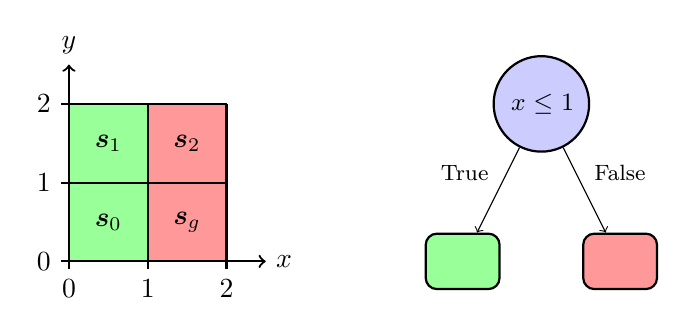
\begin{tikzpicture}[
        decision/.style={circle, draw, thick, fill=blue!20, text width=2.5em, text centered, minimum height=2.5em, font=\small},
        leaf/.style={rectangle, draw, thick, fill=green!20, text width=2em, text centered, rounded corners, minimum height=2em, font=\small},
        edge_label/.style={font=\footnotesize, midway}
    ]
        % Tree 4: if x <= 0.5 move right else move left
        \node[decision] (tree4_root) at (6,2) {$x \leq 1$};
        \node[rectangle, draw, thick, fill=green!40, text width=2em, text centered, rounded corners, minimum height=2em, font=\small] (tree4_right) at (5,0) {};
        \node[rectangle, draw, thick, fill=red!40, text width=2em, text centered, rounded corners, minimum height=2em, font=\small] (tree4_left) at (7,0) {};
        \draw[->] (tree4_root) -- (tree4_right) node[edge_label, above left] {True};
        \draw[->] (tree4_root) -- (tree4_left) node[edge_label, above right] {False};
        \tikzstyle{grid}=[draw, thick, fill=gray!10]
        
        % Draw grid
        \draw[fill=green!40] (0, 0) rectangle (1,2);
        \draw[fill=red!40] (1, 0) rectangle (2,2);

        \draw[grid] (0,0) grid (2,2);
        
        % Add axes
        \draw[thick, ->] (0,0) -- (2.5,0) node[right] {$x$};
        \draw[thick, ->] (0,0) -- (0,2.5) node[above] {$y$};
        
        % Add tick marks and labels
        \foreach \x in {0,1,2} {
            \draw[thick] (\x,0) -- (\x,-0.1) node[below] {$\x$};
        }
        \foreach \y in {0,1,2} {
            \draw[thick] (0,\y) -- (-0.1,\y) node[left] {$\y$};
        }

        \node at (0.5,0.5) {$\boldsymbol{s}_0$};
        \node at (1.5,0.5) {$\boldsymbol{s}_g$};
        \node at (1.5,1.5) {$\boldsymbol{s}_2$};
        \node at (0.5,1.5) {$\boldsymbol{s}_1$};

    \end{tikzpicture}}
    \caption{In this MDP, there are four data to which to assign either a green or red label.
    On the right, there is the unique optimal depth-1 tree for this particular MDP. This depth-1 tree also maximizes the accuracy on the corresponding classification task.}\label{example:cmdp}
    \end{figure}

\begin{figure}
    \centering
    \includegraphics[width=0.4\textwidth]{../slides_soutenance/tree_distributions_merged.pdf}
    \caption{We reproduce the same plot as in figure~\ref{fig:dt-distrib-poibmdp} for POIBMDPs associated to a downstream MDP encoding a classification task. Each colored dot is the number of final learned trees with a specific structure for a given $\zeta$.}\label{fig:tree-distrib-classif-poibmdp}
\end{figure}

\section{Discussion}
In this paper, we were interested in algorithms that can learn decision tree policies that directly optimize some trade-off of interpretability and performance in MDPs without relying on an oracle or expert policy.
Starting from the IBMDP formulation from~\citet{topin2021iterative}, we have shown that direct learning of decision tree policies for MDPs can be framed as learning deterministic memoryless policies in POMDPs that we called POIBMDPs.
By bridging the gap with the POMDP literature, we conjectured that partial observability is the main limitation for reinforcement learning of decision tree policies for MDPs.
We then supported this conjecture by benchmarking different reinforcement learning algorithms on carefully crafted problems for which we knew the exact optimal decision tree policies.
Across our experiments, we found that only when partial observablity is absent from the learning task can good decision tree policies be trained.
Attempting to overcome the partial observability challenges highlighted so far seems like a bad research direction.
Indeed, while algorithms tailored specifically for the problem of learning deterministic memoryless policies for POIBMDPs might exist, imitation learning works well in practice and has been the state-of-the-art for interpretable sequential decision making for a while.
Furthermore there are other limitations that we did not cover in the framework of~\citet{topin2021iterative} such as how to choose good candidates information-gathering actions or simply how to choose $\zeta$ for a target interpretability-performance trade-off.
Finally, while we focused on non-parametric tree learning assuming RL algorithms should naturally trade off interpretability and performance through the reward signal $\zeta$ for adding nodes to the decision tree policy, another future research avenue could be to develop better algortihms training parametric trees.
Indeed parametric tree policies, on the other hand, can be computed with reinforcement learning directly in the downstream MDP.
However such RL algorithms for parametric decision tree policies~\cite{silva,vos2024optimizinginterpretabledecisiontree,sympol} require to re-train a policy entirely for each desired level of interpretability, i.e. each unique tree structure.
Future research in this direction should focus on algorithms for parametric tree policies that can re-use samples from one tree learning to train a different tree structure more efficiently.
This would reduce the required quantity of a priori knowledge on the decision tree policy structure.
\section*{Impact statement}
Our work put great emphasis on covering existing work, open sourcing code, and being transparent about limitations.
We hope that the impact of our work is going to be positive for society through advancing reseach in interpretable machine learning.
\bibliography{example_paper}
\bibliographystyle{icml2026}

%%%%%%%%%%%%%%%%%%%%%%%%%%%%%%%%%%%%%%%%%%%%%%%%%%%%%%%%%%%%%%%%%%%%%%%%%%%%%%%
%%%%%%%%%%%%%%%%%%%%%%%%%%%%%%%%%%%%%%%%%%%%%%%%%%%%%%%%%%%%%%%%%%%%%%%%%%%%%%%
% APPENDIX
%%%%%%%%%%%%%%%%%%%%%%%%%%%%%%%%%%%%%%%%%%%%%%%%%%%%%%%%%%%%%%%%%%%%%%%%%%%%%%%
%%%%%%%%%%%%%%%%%%%%%%%%%%%%%%%%%%%%%%%%%%%%%%%%%%%%%%%%%%%%%%%%%%%%%%%%%%%%%%%
\newpage
\appendix
\onecolumn
\section{From a policy to a tree}
\begin{algorithm}[t]
    \KwData{Deterministic partially observable policy $\pi_{po}$ for IBMDP $\mathcal{M}_{IB}\equiv \langle S \times O,A \cup A_{info}, (R, \zeta), (T_{info}, T, T_0)\rangle$ and IBMDP observation $\boldsymbol{o}=(L'_1, U'_1, \dots, L'_p, U'_p)$}
    \KwResult{Decision tree policy $\pi_{\mathcal{T}}$ for MDP $\mathcal{M}\equiv\langle S, A, R, T, T_0\rangle$}
    
    \SetKwProg{Fn}{Function}{:}{}
    \SetKwFunction{SubtreeFromPolicy}{Subtree\_From\_Policy}
    
    \Fn{\SubtreeFromPolicy{$\boldsymbol{o}, \pi_{po}$}}{
        $a \leftarrow \pi_{po}(\boldsymbol{o})$ \\
        \If{$a$ is a downstream action}{
            \Return Leaf\_Node(action: $a$)
        }
        \Else{
            $\langle i, v\rangle \leftarrow a$\\
            $\boldsymbol{o}_L \leftarrow \boldsymbol{o}; \quad \boldsymbol{o}_R \leftarrow \boldsymbol{o}$ \\
                         $\boldsymbol{o}_L \leftarrow (L'_1, U'_1, \dots, L'_j, v, \dots, L'_p, U'_p); \quad \boldsymbol{o}_R \leftarrow (L'_1, U'_1, \dots, v, U'_j, \dots, L'_p, U'_p)$ \\
            $child_L \leftarrow$ Subtree\_From\_Policy$(\boldsymbol{o}_L, \pi_{po})$ \\
            $child_R \leftarrow$ Subtree\_From\_Policy$(\boldsymbol{o}_R, \pi_{po})$ \\
            \Return Internal\_Node(feature: $i$, value: $v$, children: $(child_L, child_R)$)
        }
    }
    \caption{Extract a decision tree policy (algorithm 1 from~\citet{topin2021iterative})}\label{alg:extract-tree}
\end{algorithm}

\section{Imitation learning: a baseline for indirect decision tree policy learning}\label{sec:imit}
In this section we present decision tree policies of this manuscript obtained using Dagger or VIPER~\cite{viper,pirl} after learning an expert Q-function for the grid world MDP.
Recall the optimal policies for the grid world, taking the green actions in each state in figure~\ref{fig:mdp-dt}. 
Among the optimal policies, the ones that go left or up in the goal state can be problematic for imitation learning algorithms.
Indeed, we know that for this grid world MDP there exists decision tree policies with a very good interpretability-performance trade-off: depth-1 decision trees that are optimal w.r.t. the RL objective.
One could even say that those trees have the \textit{optimal} interpretability-performance trade-off because they are the shortest trees that are optimal w.r.t. the RL objective.

In figure~\ref{fig:trees-intro}, we present a depth-1 decision tree policy that is optimal w.r.t. the RL objective and a depth-1 tree that is sub-optimal.
The other optimal depth-1 tree is to go right when $y\leq 1$ and down otherwise.

Now a fair question is: can Dagger or VIPER learn such an optimal depth-1 tree given access to an expert optimal policy from figure~\ref{fig:mdp-dt}?

We start by running the standard Q-learning algorithm with $\epsilon=0.3$, $\alpha=0.1$ over 10,000 time steps.
While for Q-learning, Sutton and Barto break ties by index value in their book~\cite{sutton} (the greedy action is the $\operatorname{argmax}$ action with smallest index), we show that the choice of tie-breaking greatly influences the performance of subsequent imitation learning algorithms.
Indeed, depending on how actions are ordered in practice, Q-learning may be biased toward some optimal policies rather than others.
While this does not matter for one who just wants to find an optimal policy, in our example of finding the optimal depth-1 decision tree policy, it matters \textit{a lot}.

In the left plot of figure~\ref{fig:ql-il}, we see that Q-learning, independently of how ties are broken, consistently converges to an optimal policy over 100 runs (random seeds).
However, in the right plot of figure~\ref{fig:ql-il}, where we plot the proportion over 100 runs of optimal decision trees returned by Dagger or VIPER at different stages of Q-learning, we observe that imitating the optimal policy obtained by breaking ties at random consistently yields more optimal trees than breaking ties by indices.
What actually happens is that the most likely output of Q-learning when ties are broken by indices is the optimal policy that goes left in the goal state,
which cannot be perfectly represented by a depth-1 decision tree, because there are three different actions taken and a binary tree of depth $D=1$ can only map to $2^D=2$ labels.

This short experiment shows that imitation learning approaches can sometimes be very bad at learning decision tree policies with good interpretability-performance trade-offs for very simple MDPs. 
Despite VIPER almost always finding the optimal depth-1 decision tree policy in terms of the RL objective when ties are broken at random, we have shed light on the sub-optimality of indirect approaches such as imitation learning.
This motivates the study of direct approaches to directly search for policies with good interpretability-performance trade-offs with respect to the original RL objective.

\begin{figure}
    \centering
    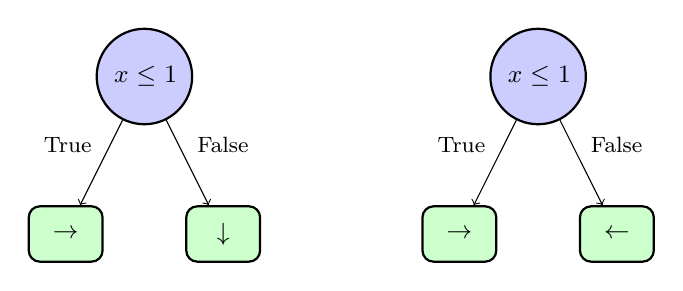
\begin{tikzpicture}[
        decision/.style={circle, draw, thick, fill=blue!20, text width=2.5em, text centered, minimum height=2.5em, font=\small},
        leaf/.style={rectangle, draw, thick, fill=green!20, text width=2em, text centered, rounded corners, minimum height=2em, font=\small},
        edge_label/.style={font=\footnotesize, midway}
    ]
        % Tree 4: if x <= 0.5 move right else move left
        \node[decision] (tree4_root) at (10,2) {$x \leq 1$};
        \node[leaf] (tree4_right) at (9,0) {$\rightarrow$};
        \node[leaf] (tree4_left) at (11,0) {$\leftarrow$};
        \draw[->] (tree4_root) -- (tree4_right) node[edge_label, above left] {True};
        \draw[->] (tree4_root) -- (tree4_left) node[edge_label, above right] {False};
        \tikzstyle{grid}=[draw, thick, fill=gray!10]


        % Tree 4: if x <= 0.5 move right else move left
        \node[decision] (tree5_root) at (5,2) {$x \leq 1$};
        \node[leaf] (tree5_right) at (4,0) {$\rightarrow$};
        \node[leaf] (tree5_left) at (6,0) {$\downarrow$};
        \draw[->] (tree5_root) -- (tree5_right) node[edge_label, above left] {True};
        \draw[->] (tree5_root) -- (tree5_left) node[edge_label, above right] {False};
        \tikzstyle{grid}=[draw, thick, fill=gray!10]

    \end{tikzpicture}
    \caption{Left, an optimal depth-1 decision tree policy for the grid world MDP from figure~\ref{fig:mdp-dt}. On the right, a sub-optimal depth-1 decision tree policy.}\label{fig:trees-intro}
    \end{figure}

\begin{figure}
    \centering
    \includegraphics[width=1\textwidth]{../images/images_part1/base_mdp.pdf}
    \caption{Left, sample complexity curve of Q-learning with default hyperparameters on the $2\times 2$ grid world MDP over 100 random seeds. Right, performance of indirect interpretable methods when imitating the greedy policy with a tree at different Q-learning stages.}\label{fig:ql-il}
\end{figure}

\section{Reproducing ``Iterative Bounding MDPs: Learning Interpretable Policies via Non-Interpretable Methods''}\label{sec:reprod}
We attempt to reproduce the results from~\cite{topin2021iterative} in which authors compare direct and indirect learning of decision tree policies of depth at most 2 for the CartPole MDP~\cite{cartpole}.
In the original paper, the authors find that both direct and indirect learning yields decision tree policies with similar RL objective values (definition~\ref{def:mdp-obj}) for the CartPole.
On the other hand, we find that, imitation learning, despite not directly optimizing the RL objective for CartPole, outperforms deep RL which directly optimizes a trade-off of the standard RL objective and interpretability.

Authors of~\citet{topin2021iterative} use two deep reinforcement learning baselines to which they apply some modifications in order to learn memoryless policies.
Authors modify the standard DQN~\cite{DQN} to return a memoryless policy. The trained $Q$-function is approximated with a neural network $O\rightarrow \mathbb{R}^{|A\cup A_{info}|}$ rather than $S\times O\rightarrow \mathbb{R}^{|A\cup A_{info}|}$.
In this modified DQN, the temporal difference error target for the $Q$-function $O\rightarrow A\cup A_{info}$ is approximated by a neural network $S\times O\rightarrow A\cup A_{info}$ that is in turn trained by bootstrapping the temporal difference error with itself.
We present the modifications in algorithm~\ref{alg:mod-dqn}.
Similar modifications are applied to the standard PPO~\cite{ppo} that we present in the appendix (algorithm \ref{alg:mod-ppo}). In the modified PPO, neural network policy $O\rightarrow A\cup A_{info}$ is trained using a neural network value function $S\times O\rightarrow A\cup A_{info}$ as a critic.

Those two variants of DQN and PPO have first been introduced in \cite{pinto} for robotic tasks with partially observable components, under the name ``asymmetric'' actor-critic. 
Asymmetric RL algorithms that have policy and value estimates using different information from a POMDP~\cite{POMDP,chap2} were later studied theoretically to solve POMDPs in Baisero's work~\cite{baisero-dqn,baisero-ppo}.
The connections from Deep RL in IBMDPs for objective is absent from \cite{topin2021iterative} and we defer their connections to direct interpretable reinforcement learning to the next chapter as our primary goal is to reproduce \cite{topin2021iterative} \textit{as is}.
Next, we present the precise experimental setup we use to reproduce~\cite{topin2021iterative} in order to study direct deep reinforcement learning of decision tree policies for the CartPole MDP.

\subsection{IBMDP formulation}\label{sec:ibmdp-paper}
Given a base MDP $\mathcal{M}\equiv\langle S, A, R, T, T_0\rangle$ (cf. definition~\ref{def:mdp}), in order to define an IBMDP $\mathcal{M}_{IB}\langle S\times O, A\cup A_{info}, (R, \zeta),( T, T_0, T_{info})\rangle$ (cf. definition~\ref{def:ibmdp}), the user needs to provide the set of information gathering actions $A_{info}$ and the reward $\zeta$ for taking those.
Authors of~\citer{topin2021iterative} propose to parametrize the set of IGAs with $j \times q$ actions $\langle j, v_k \rangle$ with $v_k$ depending on the current observation $\boldsymbol{o}_t=(L'_1, U'_1, \dots, L'_j, U'_j, \dots, L'_p, U'_p)$: $v_k = \frac{k(U'_j - L'_j)}{q+1}$.
This parametric IGAs space keeps the discrete IBMDP action space at a reasonable size while providing a learning algorithm with varied IGAs to try.

For example, if we define an IBMDP with $q=3$ for the grid world from figure~\ref{fig:mdp-dt}, the grid world action space is augmented with six IGAs. 
At $t=0$, recall that $\boldsymbol{o}_0=(0, 2, 0, 2)$, so if an IGA is taken, e.g. $\langle 2, v_2\rangle$, the effective IGA is $\langle j, v_2=\frac{k(2-0)}{3+1}\rangle = \langle 1, 2 \rangle$ which in turn effectively corresponds to an internal decision tree node $y \leq 1$.
If the current state $y$-feature value is $0.5$, then the next observation at $t=1$ is $\boldsymbol{o}_1=(0, 2, 0, 1)$. At $t=2$ if $a_t=\langle 2, v_2 \rangle$ again, it would be effectively $\langle j, v_2=\frac{k(1-0)}{3+1}\rangle = \langle 2, 0.5 \rangle$. 
This would give the next observation at $t=2$ $\boldsymbol{o}_2=(0, 2, 0, 0.5)$ and so on. 

Furthermore, author propose to regularize the learned decision tree policy with a maximum depth parameter $D$.
Unfortunately, the authors did not describe how they implemented the depth control in their work, hence we have to try different approaches to reproduce their results.

To control the tree depth during learning in the IBMDP, we can either give negative reward for taking $D$ IGAs in a row, or terminate the trajectory.
In practice, we could also have a state-dependent action space such that taking an IGA is not allowed after taking $D$ IGAs in a row.
The latter approach--sometimes called action masking--is not compatible with the definition of an MDP (cf. definition~\ref{def:mdp}) in which all actions are available in all states. 
To apply the penalization approaches, one can extend the MDP states to keep track of the current tree depth.
Similarly, the termination approach requires a transition function that depends on the current tree depth.

We actually find that when $q+1$, the parameter that defines threshold values in decision tree policy nodes (cf. definition~\ref{def:ibmdp}), is a prime number, then as a direct consequence of the \textit{Chinese Remainder Theorem}\footnote{\url{https://en.wikipedia.org/wiki/Chinese_remainder_theorem}}, the current tree depth is directly encoded in the current observation $\boldsymbol{o}_t$. 
Hence, when $q+1$ is prime, we can control the depth through either transitions or rewards without tracking the tree depth.
We use the exact same downstream MDP and associated IBMDPs for our experiments as~\cite{topin2021iterative} except when mentioned otherwise.

\paragraph{downstream MDP} The task at hand is to optimize the RL objective (definition~\ref{def:mdp-obj}) with a decision tree policy for the CartPole MDP~\cite{cartpole}.
At each time step a learning algorithm observes the cart's position and velocity and the pole's angle and angular velocity, and can take action to push the CartPole left or right.
While the CartPole is roughly balanced, i.e., while the cart's angle remains in some fixed range, the agent gets a positive reward.
If the CartPole is out of balance, the MDP transitions to an absorbing terminal state and gets 0 reward forever.
Like in~\cite{topin2021iterative}, we use the gymnasium \texttt{CartPole-v0} implementation~\cite{gymnasium} of the CartPole MDP in which trajectories are truncated after 200 timesteps making the maximum cumulative reward, i.e. the optimal value of the RL objective when $\gamma=1$, to be 200.
The state features of the CartPole MDP are in $[-2, 2] \times [-2, 2] \times [-0.14, 0.14] \times [-1.4, 1.4]$.

\paragraph{IBMDP} Authors define the associated IBMDP (definition~\ref{def:ibmdp}) with $\zeta=-0.01$ and 4 information gathering actions.
In addition to the original IBMDP paper, we also try $\zeta=0.01$ and 3 information gathering actions.
We use the same discount factor as the authors: $\gamma=1$.
We try two different approaches to limit the depth of decision tree policies to be at most 2: terminating trajectories if the agent takes too many information gathering actions in a row or simply giving a reward of $-1$ to the agent every time it takes an information gathering action past the depth limit.
In practice, we could have tried an action masking approach, i.e. having a state dependent-action set, but we want to abide to the MDP formalism in order to properly understand direct interpretable approaches.
We will also try IBMDPs where we do not limit the maximum depth for completeness.

\begin{table}[H]
    \centering
    \caption{IBMDP hyperparameters. We try 12 different IBMDPs. In green we highlight the hyperparameters from the original paper and in red we highlight the hyperparameter names for which author do not give information.}\label{tab:ibmdp-params}
    \begin{tabular}{ll}
    \toprule
    \textbf{Hyperparameter} & \textbf{Values}\\
    \midrule
    Discount factor $\gamma$ & \textcolor{green}{1} \\
    Information gathering actions parameter $q$ & 2, \textcolor{green}{3} \\
    Information gathering actions rewards $\zeta$ & \textcolor{green}{-0.01}, 0.01 \\
    \textcolor{red}{Depth control} & Done signal, negative reward, none \\ 
    \bottomrule
    \end{tabular}
    \end{table}


\begin{table}[H]
    \centering
    \caption{(Modified) DQN trained on $10^6$ timesteps. This gives four different instantiation of (modified) DQN. Hyperparameters not mentioned are stable-baselines3 default. In green we highlight the hyperparameters from the original paper and in red we highlight the hyperparameter names for which author do not give information.}\label{tab:ibmdp-rl1}
    \begin{tabular}{ll}
    \toprule
    \textbf{Hyperparameter} & \textbf{Values}\\
    \midrule
    Buffer size & \textcolor{green}{$10^6$} \\
    Random transitions before learning & \textcolor{green}{$10^5$} \\
    Epsilon start & 0.9, \textcolor{green}{0.5} \\
    Epsilon end & \textcolor{green}{0.05} \\
    Exploration fraction & \textcolor{green}{0.1} \\
    Optimizer & \textcolor{green}{RMSprop ($\alpha = 0.95$)}\\
    Learning rate & \textcolor{green}{$2.5\times10^{-4}$}\\
    Networks architectures & \textcolor{green}{[128, 128]}\\
    \textcolor{red}{Networks activation} & $\operatorname{tanh()}$, $\operatorname{relu()}$\\
    \bottomrule
    \end{tabular}
    \end{table}

\begin{table}[H]
    \centering
    \caption{(Modified) PPO trained on $4\times10^6$ timesteps. This gives two different instantiation of (modified) PPO. Hyperparameters not mentioned are stable-baselines3 default. In green we highlight the hyperparameters from the original paper and in red we highlight the hyperparameter names for which author do not give information.}\label{tab:ibmdp-rl2}
    \begin{tabular}{ll}
    \toprule
    \textbf{Hyperparameter} & \textbf{Values}\\
    \midrule
    Steps between each policy gradient steps & \textcolor{green}{512} \\
    Number of minibatch for policy gradient updates & \textcolor{green}{4} \\
    Networks architectures & \textcolor{green}{[64, 64]}\\
    \textcolor{red}{Networks activations} & $\operatorname{tanh()}$, $\operatorname{relu()}$\\
    \bottomrule
    \end{tabular}
    \end{table}


In tables~\ref{tab:mod-dqn} and~\ref{tab:mod-ppo} we report the top-5 hyperparameters for Modified RL baselines when learning partially observable IBMDP policies in terms of extracted decision tree policies performances in the CartPole MDP.
\begin{table}
    \centering
    \caption{Top 5 hyperparameter configurations for modified DQN + IBMDP, bold font represent the original paper hyperparameters.}\label{tab:mod-dqn}
    \label{tab:top5_results}
    \begin{tabular}{ccccccS}
    \toprule
    Rank & $q$ & Depth control & Activation & Exploration & $\zeta$ & {Mean Final Performance} \\
    \midrule
    1 & 3 & termination & $\operatorname{tanh}$ & 0.9 & 0.01 & 53 \\
    2 & 2 & termination & $\operatorname{tanh}$ & 0.5 & -0.01 & 24 \\
    \textbf{3} & \textbf{3} & \textbf{termination} & $\operatorname{tanh}$ & \textbf{0.5} & \textbf{-0.01} & \textbf{24} \\
    4 & 2 & termination & $\operatorname{tanh}$ & 0.5 & 0.01 & 23 \\
    5 & 2 & termination & $\operatorname{tanh}$ & 0.9 & -0.01 & 22 \\
    \bottomrule
    \end{tabular}
    \end{table}

    \begin{table}
        \centering
        \caption{Top 5 hyperparameter configurations for modified PPO + IBMDP, bold font represent the original paper hyperparameters.}\label{tab:mod-ppo}
        \label{tab:top5_ppo_results}
        \begin{tabular}{cccccS}
        \toprule
        Rank & $q$ & Depth Control & Activation & $\zeta$ & {Mean Final Performance} \\
        \midrule
        1 & 3 & reward & $\operatorname{relu}$ & 0.01 & 139 \\
        2 & 3 & termination & $\operatorname{relu}$ & 0.01 & 132 \\
        \textbf{3} & \textbf{3} & \textbf{reward} & $\operatorname{tanh}$ & \textbf{-0.01} & \textbf{119} \\
        4 & 3 & reward & $\operatorname{relu}$ & -0.01 & 117 \\
        5 & 3 & reward & $\operatorname{tanh}$ & 0.01 & 116 \\
        \bottomrule
        \end{tabular}
        \end{table}


\begin{algorithm}
    \KwData{IBMDP $\mathcal{M}_{IB}\langle S\times O, A\cup A_{info}, (R, \zeta),( T, T_0, T_{info})\rangle$, learning rate $\alpha$, exploration rate $\epsilon$, partially observable Q-network parameters $\theta$, Q-network parameters $\phi$, replay buffer $\mathcal{B}$, update frequency $C$}
    \KwResult{deterministic memoryless policy $\pi_{po}$}
    Initialize partially observable Q-network parameters $\theta$\\
    \textcolor{teal}{Initialize Q-network parameters $\phi$ and target network parameters $\phi^- = \phi$} \\

    Initialize replay buffer $\mathcal{B} = \emptyset$ \\
    \For{each episode}{
        Initialize downstream state features $\boldsymbol{s}_0 \sim T_0$ \\
        Initialize observation $\boldsymbol{o}_0 = (L_1, U_1, \dots, L_p, U_p)$ \\

        \For{each step $t$}{
            Choose action $a_t$ using $\epsilon$-greedy: $a_t = \operatorname{argmax}_a Q_\theta(\boldsymbol{o}_t,a)$ with prob. $1-\epsilon$ \\
            Take action $a_t$, observe $r_t$ \\
            Store transition $(\boldsymbol{s}_t, \boldsymbol{o}_t, a_t, r_t, \boldsymbol{s}_{t+1})$ in $\mathcal{B}$ \\
            Sample random batch $(\boldsymbol{s}_i, \boldsymbol{o}_i, a_i, r_i, \boldsymbol{s}_{i+1}) \sim \mathcal{B}$ \\
            $a' = \underset{a}{\operatorname{argmax}} Q_{\theta}(\boldsymbol{o}_i, a)$ \\
            \textcolor{teal}{$y_i = r_i + \gamma Q_{\phi^-}(\boldsymbol{s}_{i+1}, a')$} \Comment{// Compute target}
            $\phi \leftarrow \phi - \alpha \nabla_\phi (Q_\phi(\boldsymbol{s}_i, a_i) - y_i)^2$ \Comment{// Update Q-network}
            \textcolor{teal}{$\theta \leftarrow \theta - \alpha \nabla_\theta (Q_\theta(\boldsymbol{o}_i, a_i) - y_i)^2$} \Comment{// Update partially observable Q-network}

            \If{$t \bmod C = 0$}{
                $\theta^- \leftarrow \theta$ \Comment{// Update target network}
            }
            $\boldsymbol{s}_t \leftarrow \boldsymbol{s}_{t+1}$ \\
            $\boldsymbol{o}_t \leftarrow \boldsymbol{o}_{t+1}$ \\
        }
    }
    $\pi_{po}(\boldsymbol{o}) = \operatorname{argmax}_a Q_\theta(\boldsymbol{o},a)$ \Comment{// Extract greedy policy}
    \caption{Modified Deep Q-Network. We highlight in green the changes to the standard DQN~\cite{dqn}.}\label{alg:mod-dqn}
\end{algorithm}

\begin{algorithm}
    \KwData{IBMDP $\mathcal{M}_{IB}\langle S\times O, A\cup A_{info}, (R, \zeta),( T, T_0, T_{info})\rangle$, learning rate $\alpha$, policy parameters $\theta$, clipping parameter $\epsilon$, value function parameters $\phi$}
    \KwResult{Memoryless stochastic policy $\pi_{po_\theta}$}
    Initialize policy parameters $\theta$ and value function parameters $\phi$ \\
    \For{each episode}{
        Generate trajectory $\tau = (\boldsymbol{s}_0, \boldsymbol{o}_0, a_0, r_0, \boldsymbol{s}_1, \boldsymbol{o}_1, a_1, r_1, \ldots)$ following $\pi_\theta$ \\
        \For{each timestep $t$ in trajectory}{
            $G_t \leftarrow \sum_{k=t}^{T} \gamma^{k-t} r_k$ \Comment{// Compute return}
            $A_t \leftarrow G_t - V_\phi(\boldsymbol{s}_t)$ \Comment{// Compute advantage}
            $r_t(\theta) \leftarrow \frac{\pi_{po_\theta}(a_t|\boldsymbol{o}_t)}{\pi_{po_\theta}_{old}(a_t|\boldsymbol{o}_t)}$ \Comment{// Compute probability ratio}
            $L^{CLIP}_t \leftarrow \min(r_t(\theta) A_t, \text{clip}(r_t(\theta), 1-\epsilon, 1+\epsilon) A_t)$ \Comment{// Clipped objective}
            $\theta \leftarrow \theta + \alpha \nabla_\theta L^{CLIP}_t$ \Comment{// Policy update}
            $\phi \leftarrow \phi + \alpha \nabla_\phi (G_t - V_\phi(\boldsymbol{s}_t))^2$ \Comment{// Value function update}
        }
        $\theta_{old} \leftarrow \theta$ \Comment{// Update old policy}
    }
    \caption{Modified Proximal Policy Optimization}\label{alg:mod-ppo}
\end{algorithm}

\subsection{Experimental setup}

\paragraph{Modified DQN and Modified PPO} as mentioned above, the authors use the modified version of DQN from algorithm~\ref{alg:mod-dqn}.
We use the exact same hyperparameters for modified DQN as the authors when possible. 
We use the same layers width (128) and number of hidden layers (2), the same exploration strategy ($\epsilon$-greedy with linearly decreasing value $\epsilon$ between 0.5 and 0.05 during the first 10\% of the training),
the same replay buffer size ($10^6$) and the same number of transitions to be collected randomly before doing value updates ($10^5$).
We also try to use more exploration during training (change the initial $\epsilon$ value to 0.9).
We use the same optimizer (RMSprop with hyperparameter 0.95 and learning rate $2.5 \times 10^{-4}$) to update the $Q$-networks.
Authors did not share which DQN implementation they used so we use the stable-baselines3 one~\cite{stable-baselines3}\footnote{We are cleaning our source code and will open source it as soon as possible}.
Authors did not share which activation functions they used so we try both $\operatorname{tanh}$ and $\operatorname{relu}$. 
For the modified PPO algorithm (algorithm~\ref{alg:mod-ppo}), we can exactly match the authors hyperparameters since they use the open source stable-baselines3 implementation of PPO.
We match training budgets: we train modified DQN on 1 million timesteps and modified PPO on 4 million timesteps.

\paragraph{DQN and PPO} We also benchmark the standard DQN and PPO when learning standard Markovian IBMDP policies $\pi:S\times O\rightarrow A\cup A_{info}$ and when learning standard $\pi:S\rightarrow A$ policies directly in the CartPole MDP.
We summarize hyperparameters for the IBMDP and for the learning algorithms in appendices~\ref{tab:ibmdp-params}, \ref{tab:ibmdp-rl1} and \ref{tab:ibmdp-rl2}.

\paragraph{Indirect methods} We also compare modified RL algorithm to imitation learning.
To do so, we use VIPER or Dagger to imitate greedy neural network policies obtained with standard DQN learning directly on CartPole.
We use Dagger to imitate neural network policies obtained with the standard PPO learning directly on CartPole. 
For each indirect method, we imitate the neural network experts by fitting decision trees on 10000 expert transitions using the CART~\cite{breiman1984classification} implementation from scikit-learn~\cite{scikit-learn} with default hyperparameters and maximum depth of 2 like in ~\cite{topin2021iterative}.
    
\subsubsection{Metrics}
The key metric of this section is performance when controlling the CartPole, i.e, the average \textit{undiscounted} cumulative reward of a policy on 100 trajectories (RL objective with $\gamma=1$).
For modified RL algorithms that learn a memoryless policy (or $Q$-function) in an IBMDP, we periodically extract the policy (or $Q$-function) and use algorithm~\ref{alg:extract-tree} to extract a decision tree for the CartPole MDP. 
We then evaluate the tree on 100 independent trajectories in the MDP and report the mean undiscounted cumulative reward.
For RL applied to IBMDPs, since we can't deploy learned policies directly to the downstream MDP as the state dimensions mismatch--such policies are $S\times O\rightarrow A \cup A_{info}$ but the MDP states are in $S$--we periodically evaluate those IBMDP policies in a copy of the IBMDP in which we fix $\zeta=0$ ensuring that the copied IBMDP undiscounted cumulative rewards only account rewards from the CartPole MDP (non-zero rewards in the IBMDP only occur when a reward from the downstream MDP is given, i.e. when $a_t\in A$ in the IBMDP (definition~\ref{def:ibmdp})).
Similarly, we do 100 trajectories of the extracted policies in the copied IBMDP and report the average undiscounted cumulative reward.
For RL applied directly to the downstream MDP we can just periodically extract the learned policies and evaluate them on 100 CartPole trajectories.

Since imitation learning baselines train offline, i.e, on a fixed dataset, their performances cannot directly be reported on the same axis as RL baselines.
For that reason, during the training of a standard RL baseline, we periodically extract the trained neural policy/$Q$-function that we consider as the expert to imitate.
Those experts are then imitated with VIPER or Dagger using 10 000 newly generated transitions and then fitsted decision tree policies are then evaluated on 100 CartPole trajectories.
We do not report the imitation learning objective values during VIPER or Dagger training.
Every single combination of IBMDP and Modified RL hyperparameters is run 20 times.
For standard RL on either an IBMDP or an MDP, we use the paper original hyperparameters when they were specified, with depth control using negative rewards, $\operatorname{tanh()}$ activations.
We use 20 individual random seeds for every experiment in this chapter.
Next, we present our results when reproducing~\cite{topin2021iterative}.

\subsection{Results}

\subsubsection{How well do modified deep RL baselines learn in IBMDPs?}

\begin{figure*}
    \centering
    \begin{subfigure}[b]{0.49\textwidth}
        \centering
        \includegraphics[width=\textwidth]{../images/images_part1/dqn.pdf}
        \caption{DQN variants}\label{fig:res-dqn}
    \end{subfigure}
    \hfill
    \begin{subfigure}[b]{0.49\textwidth}
        \centering
        \includegraphics[width=\textwidth]{../images/images_part1/ppo.pdf}
        \caption{PPO variants}\label{fig:res-ppo}
    \end{subfigure}
    \caption{Comparison of modified reinforcement learning algorithms on different CartPole IBMDPs. (a) Shows variations of modified DQN and DQN (table~\ref{tab:ibmdp-rl1}), while (b) shows variations of modified PPO and PPO (table~\ref{tab:ibmdp-rl2}). For both algorithms, we give different line-styles for the learning curves when applied directly on the CartPole MDP versus when applied on the IBMDP to learn standard Markovian policies. We color the modified RL algorithm variant from the original paper in black. Shaded areas represent the confidence interval at 95\% at each measure on the y-axis.}
\end{figure*}
On figure~\ref{fig:res-dqn}, we observe that modified DQN can learn in IBMDPs--the curves have an increasing trend--but we also observe that modified DQN finds poor decision tree policies for the CartPole MDP in average--the curves flatten at the end of the x-axis and have low y-values.
In particular, the highest final y-value, among all the learning curves that could possibly correspond to the original paper modified DQN, correspond to poor performances on the CartPole MDP.
On figure~\ref{fig:res-ppo}, we observe that modified PPO finds decision tree policies with almost 150 cumulative rewards towards the end of training.
The performance difference with modified DQN could be because we trained modified PPO longer, like in the original paper.
However it could also be because DQN-like algorithms with those hyperparameters struggle to learn in CartPole (IB)MDPs.
Indeed, we notice that for DQN-like baselines, learning seems difficult in general independently of the setting.
On figures~\ref{fig:res-dqn} and~\ref{fig:res-ppo}, we observe that standard RL baselines (RL + IBMDP and RL + MDP), learn better CartPole policies in average than their modified counterparts that learn memoryless policies. 
On figure~\ref{fig:res-ppo}, it is clear that for the standard PPO baselines, learning is super efficient and algorithms learn optimal policies with reward 200 in few thousands steps.

\subsubsection{Which decision tree policies does direct reinforcement learning return for the CartPole MDP?}

\begin{figure}
    \centering
    \includegraphics[width=1\textwidth]{../images/images_part1/ppo_tree_study.pdf}
    \caption{(left) Mean performance of the best--w.r.t. the RL objective for CartPole--modified RL + IBMDP combination. Shaded areas represent the min and max performance over the 20 seeds during training. (right) Corresponding score distribution of the final decision tree policies w.r.t. the RL objective for CartPole.}\label{fig:ppo-trees}
\end{figure}


\begin{figure}
    \centering
    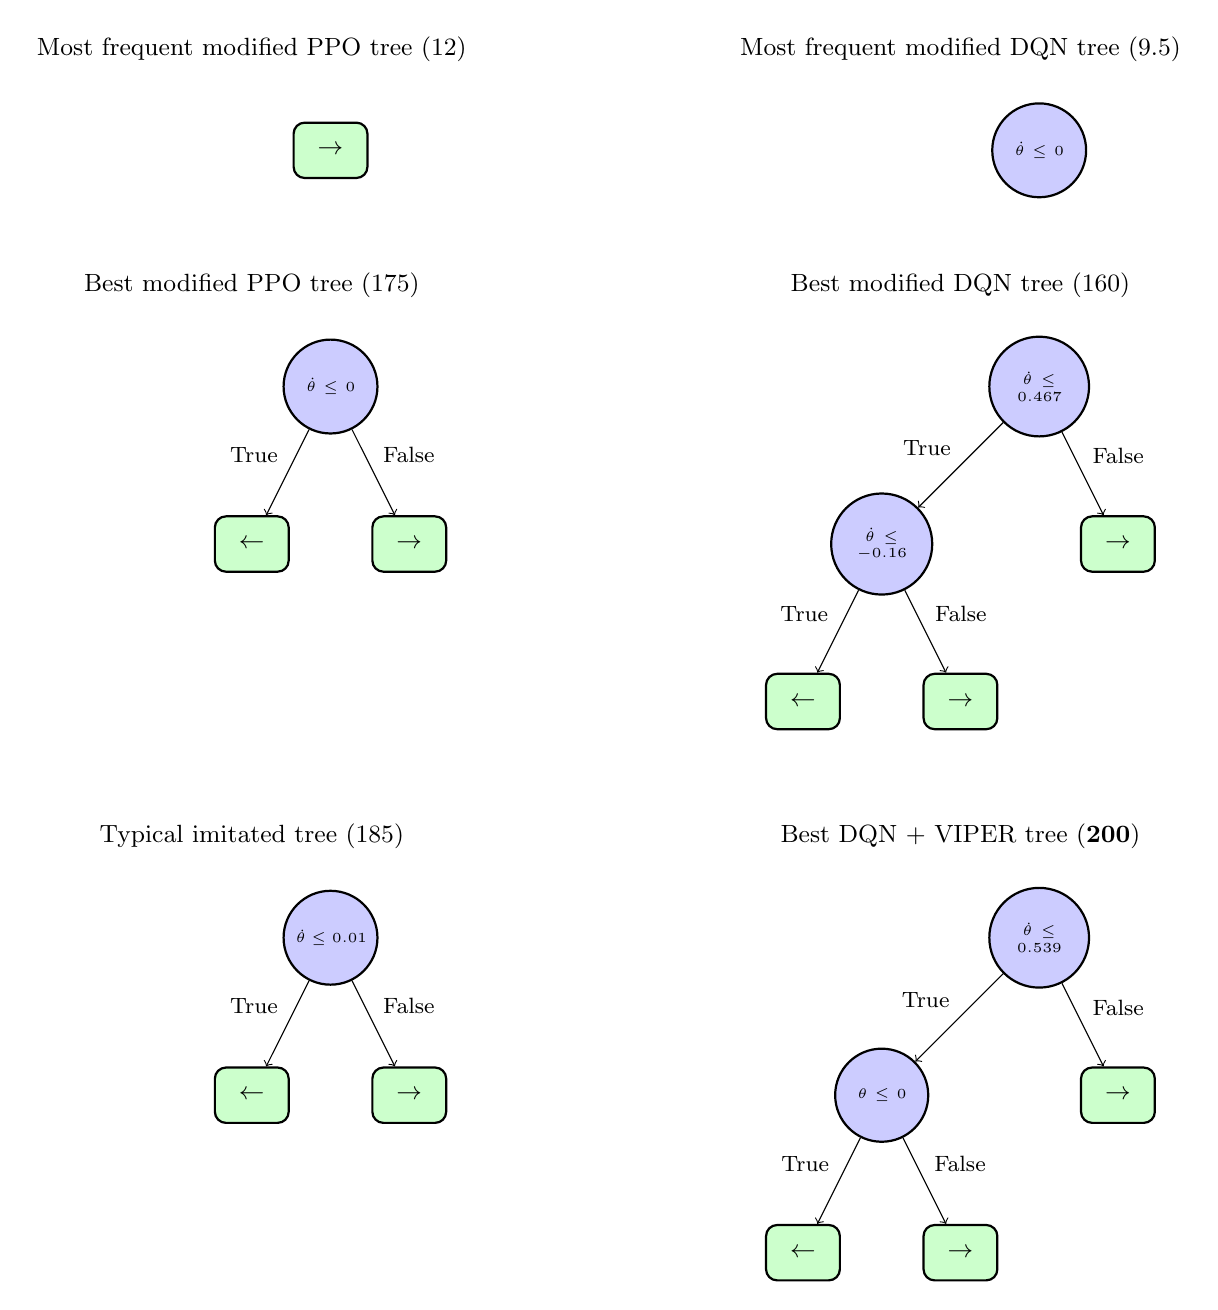
\begin{tikzpicture}[
        decision/.style={circle, draw, thick, fill=blue!20, text width=2.5em, text centered, minimum height=2.5em, font=\tiny},
        leaf/.style={rectangle, draw, thick, fill=green!20, text width=2em, text centered, rounded corners, minimum height=2em, font=\small},
        edge_label/.style={font=\footnotesize, midway}
    ]

        \node[leaf] (tree7_root) at (-3,3) {$\rightarrow$};
        % \draw[->] (tree7_root) to[out=45,in=0,looseness=5] (tree7_root);

        \node[decision] (tree7_root) at (6,3) {$\dot{\theta} \leq 0$};
        % \draw[->] (tree7_root) to[out=45,in=0,looseness=5] (tree7_root);
        
        % Tree 4: if x <= 0.5 move right else move left
        \node[decision] (tree4_root) at (-3,0) { $\dot{\theta}\leq 0$};
        \node[leaf] (tree4_right) at (-4,-2) {$\leftarrow$};
        \node[leaf] (tree4_left) at (-2,-2) {$\rightarrow$};
        \draw[->] (tree4_root) -- (tree4_right) node[edge_label, above left] {True};
        \draw[->] (tree4_root) -- (tree4_left) node[edge_label, above right] {False};
        

        % Tree 7: if x <= 0.5 and y <= 0.5 move right else move down
        \node[decision] (tree7_root) at (6,0) {$\dot{\theta}\leq 0.467$};
        \node[decision] (tree7_y) at (4,-2) {$\dot{\theta}\leq -0.16$};
        \node[leaf] (tree7_right) at (3,-4) {$\leftarrow$};
        \node[leaf] (tree7_down) at (5,-4) {$\rightarrow$};
        \node[leaf] (tree7_down2) at (7,-2) {$\rightarrow$};
        \draw[->] (tree7_root) -- (tree7_y) node[edge_label, above left] {True};
        \draw[->] (tree7_root) -- (tree7_down2) node[edge_label, above right] {False};
        \draw[->] (tree7_y) -- (tree7_right) node[edge_label, above left] {True};
        \draw[->] (tree7_y) -- (tree7_down) node[edge_label, above right] {False};




        % Tree 4: if x <= 0.5 move right else move left (Second row, left)
        \node[decision] (tree4_root2) at (-3,-7) { $\dot{\theta}\leq 0.01$};
        \node[leaf] (tree4_right2) at (-4,-9) {$\leftarrow$};
        \node[leaf] (tree4_left2) at (-2,-9) {$\rightarrow$};
        \draw[->] (tree4_root2) -- (tree4_right2) node[edge_label, above left] {True};
        \draw[->] (tree4_root2) -- (tree4_left2) node[edge_label, above right] {False};


        % Tree 7: if x <= 0.5 and y <= 0.5 move right else move down (Second row, right)
        \node[decision] (tree7_root2) at (6,-7) {$\dot{\theta}\leq 0.539$};
        \node[decision] (tree7_y2) at (4,-9) {$\theta\leq 0$};
        \node[leaf] (tree7_right2) at (3,-11) {$\leftarrow$};
        \node[leaf] (tree7_down3) at (5,-11) {$\rightarrow$};
        \node[leaf] (tree7_down4) at (7,-9) {$\rightarrow$};
        \draw[->] (tree7_root2) -- (tree7_y2) node[edge_label, above left] {True};
        \draw[->] (tree7_root2) -- (tree7_down4) node[edge_label, above right] {False};
        \draw[->] (tree7_y2) -- (tree7_right2) node[edge_label, above left] {True};
        \draw[->] (tree7_y2) -- (tree7_down3) node[edge_label, above right] {False};
        

        % Labels
        \node[above] at (-4,4) {{\small Most frequent modified PPO tree (12)}};
        \node[above] at (5,4) {{\small Most frequent modified DQN tree (9.5)}};

        \node[above] at (-4,1) {{\small Best modified PPO tree (175)}};
        \node[above] at (5,1) {{\small Best modified DQN tree (160)}};
        \node[above] at (-4,-6) {{\small Typical imitated tree (185)}};
        \node[above] at (5,-6) {{\small Best DQN + VIPER tree (\textbf{200})}};


    \end{tikzpicture}
    \caption{Trees obtained by modified deep RL in IBMDPs against trees obtained with imitation (RL objective value). $\theta$ and $\dot{\theta}$ are respectively the angle and the angular velocity of the pole}
    \label{fig:trees-drl}
\end{figure}


On figure~\ref{fig:ppo-trees}, we isolate the best performing algorithms instantiations that learn decision tree policies for the CartPole MDP.
We compare the best modified DQN and modified PPO to imitation learning baselines that use the surrogate imitation objective to find CartPole decision tree policies.
We find that despite having poor performances in \textit{average}, the modified deep reinforcement learning baselines can find very good decision tree policies as shown by the min-max shaded areas on the left of figure~\ref{fig:ppo-trees} and the corresponding estimated density of learned trees performances.
However this is not desirable, a user typically wants an algorithm that can consistently find good decision tree policies.
As shown by the estimated densities, indirect methods consistently find good decision tree policies (the higher modes of distributions are on the right of the plot).
On the other hand, the decision tree policies returned by direct RL methods seem equally distributed on both extremes of the scores.

On figure~\ref{fig:trees-drl}, we present the best decision tree policies for CartPole returned by modified DQN and modified PPO.
We used algorithm~\ref{alg:extract-tree} to extract 20 trees from the 20 memoryless policies returned by the modified deep reinforcement learning algorithms over the 20 training seeds.
We then plot the best tree for each baseline.
Those trees get an average RL objective of roughly 175.
Similarly, we plot a representative tree for imitation learning baseline as well as a tree that is optimal for CartPole w.r.t. the RL objective obtained with VIPER. 
Unlike for direct methods, the trees returned by imitation learning are extremely similar across seeds. In particular they often only vary in the scalar value used in the root node but in general have the same structure and test the angular velocity.
On the other hand the most frequent trees across seeds returned by modified RL baselines are ``trivial'' decision tree policies that either repeat the same downstream action forever or repeat the same IGA (definition~\ref{def:ibmdp}) forever.

\section{RL objective values calculations}\label{calcs}
\paragraph{Optimal depth-1 decision tree policy} $\pi_{\mathcal{T}_1}$ has one root node that tests $x\leq1$ (respectively $y\leq1$) and two leaf nodes $\rightarrow$ and $\downarrow$. 
    To compute $V^\pi_{\mathcal{T}_1}(\boldsymbol{o}_0)$, we compute the values of $\pi_{\mathcal{T}_1}$ in each of the possible starting states $(\boldsymbol{s}_0, \boldsymbol{o}_0), (\boldsymbol{s}_1, \boldsymbol{o}_0), (\boldsymbol{s}_2, \boldsymbol{o}_0), (\boldsymbol{s}_g, \boldsymbol{o}_0)$ and compute the expectation over those. 
    At initialization, when the downstream state is $\boldsymbol{s}_g = (1.5, 0.5)$, the depth-1 decision tree policy cycles between taking an information gathering action $x\leq1$ and moving down to get a positive reward for which it gets the returns:
    \begin{align*}
        V^{\pi_{\mathcal{T}_1}} (\boldsymbol{s}_g, \boldsymbol{o}_0) &= \zeta + \gamma + \gamma^2 \zeta + \gamma^3 \dots \\
        &= \overset{\infty}{\underset{t=0}\sum} \gamma^{2t} \zeta + \overset{\infty}{\underset{t=0}\sum} \gamma^{2t+1} \\
        &= \frac{\zeta + \gamma}{1 - \gamma^2}
    \end{align*}
    At initialization, in either of the downstream states $\boldsymbol{s}_0=(0.5,0.5)$ and $\boldsymbol{s}_2=(1.5, 1.5)$, the value of the depth-1 decision tree policy is the return when taking one information gathering action $x\leq1$, then moving right or down, then following the policy from the goal state $\boldsymbol{s}_g$:
    \begin{align*}
        V^{\pi_{\mathcal{T}_1}} (\boldsymbol{s}_0, o_0) &= \zeta + \gamma 0 + \gamma^2 V^{\pi_{\mathcal{T}_1}} (\boldsymbol{s}_g, o_0) \\
        &= \zeta + \gamma^2 V^{\pi_{\mathcal{T}_1}} (\boldsymbol{s}_g, o_0) \\
        &= V^{\pi_{\mathcal{T}_1}} (\boldsymbol{s}_2, o_0)
    \end{align*}
    Similarly, the value of the best depth-1 decision tree policy in state $\boldsymbol{s}_1=(0.5,1.5)$ is the value of taking one information gathering action then moving right to $\boldsymbol{s}_2$ then following the policy in $\boldsymbol{s}_2$:
    \begin{align*}
        V^{\pi_{\mathcal{T}_1}} (\boldsymbol{s}_1, \boldsymbol{o}_0) &= \zeta + \gamma 0 + \gamma^2 V^{\pi_{\mathcal{T}_1}} (\boldsymbol{s}_2, \boldsymbol{o}_0) \\
        &= \zeta + \gamma^2 V^{\pi_{\mathcal{T}_1}} (\boldsymbol{s}_2, o_0) \\
        &= \zeta + \gamma^2 (\zeta + \gamma^2 V^{\pi_{\mathcal{T}_1}} (\boldsymbol{s}_g, o_0)) \\
        &= \zeta + \gamma^2 \zeta + \gamma^4 V^{\pi_{\mathcal{T}_1}} (\boldsymbol{s}_g, o_0)
    \end{align*}
    Since the probability of being in any downstream states at initialization given that the observation is $\boldsymbol{o}_0$ is simply the probability of being in any downstream states at initialization, we can write:
    \begin{align*}
        V^{\pi_{\mathcal{T}_1}} (\boldsymbol{o}_0) &= \frac{1}{4} V^{\pi_{\mathcal{T}_1}} (\boldsymbol{s}_g, \boldsymbol{o}_0) + \frac{2}{4} V^{\pi_{\mathcal{T}_1}} (\boldsymbol{s}_2, \boldsymbol{o}_0) + \frac{1}{4} V^{\pi_{\mathcal{T}_1}} (\boldsymbol{s}_1, \boldsymbol{o}_0) \\
        &= \frac{1}{4} \frac{\zeta + \gamma}{1 - \gamma^2} + \frac{2}{4} (\zeta + \gamma^2 \frac{\zeta + \gamma}{1 - \gamma^2}) + \frac{1}{4} (\zeta + \gamma^2 \zeta + \gamma^4 \frac{\zeta + \gamma}{1 - \gamma^2}) \\
        &= \frac{1}{4} \frac{\zeta + \gamma}{1 - \gamma^2} + \frac{2}{4} (\frac{\zeta + \gamma ^ 3}{1-\gamma^2}) + \frac{1}{4}(\frac{\zeta+\gamma^5}{1-\gamma^2}) \\
        &= \frac{4\zeta + \gamma + 2\gamma^3 + \gamma^5}{4(1-\gamma^2)}
    \end{align*}

\paragraph{Depth-0 decision tree:} has only one leaf node that takes a single downstream action indefinitely.
For this type of tree the best reward achievable is to take actions that maximize the probability of reaching the objective $\rightarrow$ or $\downarrow$. In that case the objective value of such tree is:
In the goal state $G = (1, 0)$, the value of the depth-0 tree $\mathcal{T}_0$ is:
\begin{align*}
    V^{\mathcal{T}_0}_G &= 1 + \gamma + \gamma^2 + \dots \\
    &= \overset{\infty}{\underset{t=0}\sum} \gamma^t \\
    &= \frac{1}{1 - \gamma}
\end{align*}
In the state $(0, 0)$ when the policy repeats going right respectively in the state $(0, 1)$ when the policy repeats going down, the value is:
\begin{align*}
    V^{\mathcal{T}_0}_{S_0} &= 0 + \gamma V^{\mathcal{T}_0}_g \\
    &= \gamma V^{\mathcal{T}_0}_G
\end{align*}
In the other states the policy never gets positive rewards; $V^{\mathcal{T}_0}_{S_1} = V^{\mathcal{T}_0}_{S_2} = 0$. Hence:
\begin{align*}
J(\mathcal{T}_0) &= \frac{1}{4} V^{\mathcal{T}_0}_G + \frac{1}{4} V^{\mathcal{T}_0}_{S_0}+ \frac{1}{4} V^{\mathcal{T}_0}_{S_1}+ \frac{1}{4} V^{\mathcal{T}_0}_{S_2} \\
&= \frac{1}{4} V^{\mathcal{T}_0}_G + \frac{1}{4} \gamma V^{\mathcal{T}_0}_G + 0 + 0\\
&= \frac{1}{4} \frac{1}{1 - \gamma} + \frac{1}{4} \gamma \frac{1}{1 - \gamma} \\
&= \frac{1 + \gamma}{4(1 - \gamma)}
\end{align*}

\paragraph{Unbalanced depth-2 decision tree:}the unbalanced depth-2 decision tree  takes an information gathering action $x\leq0.5$ then either takes the $\downarrow$ action or takes a second information $y\leq0.5$ followed by $\rightarrow$ or $\downarrow$.
In states $G$ and $S_2$, the value of the unbalanced tree is the same as for the depth-1 tree.
In states $S_0$ and $S_1$, the policy takes two information gathering actions before taking a downstream action and so on:
\begin{align*}
    V^{\mathcal{T}_{u}}_{S_0} &= \zeta + \gamma \zeta + \gamma ^ 2 0 + \gamma ^ 3 V^{\mathcal{T}_1}_G
\end{align*} 
\begin{align*}
    V^{\mathcal{T}_{u}}_{S_1} &= \zeta + \gamma \zeta + \gamma ^ 2 0 + \gamma ^ 3 V^{\mathcal{T}_u}_{S_0} \\ 
    &= \zeta + \gamma \zeta + \gamma ^ 2 0 + \gamma ^ 3 (\zeta + \gamma \zeta + \gamma ^ 2 0 + \gamma ^ 3 V^{\mathcal{T}_1}_G) \\
    &= \zeta + \gamma \zeta + \gamma ^ 3 \zeta + \gamma ^ 4 \zeta + \gamma ^ 6 V^{\mathcal{T}_1}_G
\end{align*}
We get:
\begin{align*}
    J(\mathcal{T}_{u}) &= \frac{1}{4} V^{\mathcal{T}_u}_G + \frac{1}{4} V^{\mathcal{T}_u}_{S_0} + \frac{1}{4}V^{\mathcal{T}_u}_{S_1} + \frac{1}{4}V^{\mathcal{T}_u}_{S_2} \\
    &=  \frac{1}{4} V^{\mathcal{T}_1}_G + \frac{1}{4}(\zeta + \gamma \zeta + \gamma ^ 3 V^{\mathcal{T}_1}_G) + \frac{1}{4} (\zeta + \gamma \zeta + \gamma ^ 3 \zeta + \gamma ^ 4 \zeta + \gamma ^ 6 V^{\mathcal{T}_1}_G) + \frac{1}{4}V^{\mathcal{T}_1}_{S_2} \\
    &= \frac{1}{4} (\frac{\zeta + \gamma}{1-\gamma^2}) + \frac{1}{4}(\frac{\gamma\zeta + \gamma^4 + \zeta -\gamma^2\zeta}{1-\gamma^2}) + \frac{1}{4} (\zeta + \gamma \zeta + \gamma ^ 3 \zeta + \gamma ^ 4 \zeta + \gamma ^ 6 V^{\mathcal{T}_1}_G) + \frac{1}{4}V^{\mathcal{T}_1}_{S_2} \\
    &= \frac{1}{4} (\frac{\zeta + \gamma}{1-\gamma^2}) + \frac{1}{4}(\frac{\gamma\zeta + \gamma^4 + \zeta -\gamma^2\zeta}{1-\gamma^2}) + \frac{1}{4} (\frac{\zeta + \gamma\zeta -\gamma^2\zeta-\gamma^5\zeta+\gamma^6\zeta+\gamma^7}{1-\gamma^2}) + \frac{1}{4}V^{\mathcal{T}_1}_{S_2} \\
    &= \frac{1}{4} (\frac{\zeta + \gamma}{1-\gamma^2}) + \frac{1}{4}(\frac{\gamma\zeta + \gamma^4 + \zeta -\gamma^2\zeta}{1-\gamma^2}) + \frac{1}{4} (\frac{\zeta + \gamma\zeta -\gamma^2\zeta-\gamma^5\zeta+\gamma^6\zeta+\gamma^7}{1-\gamma^2}) + \frac{1}{4}(\frac{\zeta + \gamma ^ 3}{1-\gamma^2}) \\
    &= \frac{\zeta(4+2\gamma-2\gamma^2-\gamma^5+\gamma^6)+\gamma+\gamma^3+\gamma^4+\gamma^7}{4(1-\gamma^2)}
\end{align*}
\paragraph{The balanced depth-2 decision tree:}alternates in every state between taking the two available information gathering actions and then a downstream action.
The value of the policy in the goal state is:
\begin{align*}
    V^{\mathcal{T}_2}_{G} &= \zeta + \gamma\zeta + \gamma^2 + \gamma^3\zeta + \gamma^4\zeta + \dots \\
    &= \overset{\infty}{\underset{t=0}\sum} \gamma^{3t}\zeta + \overset{\infty}{\underset{t=0}\sum} \gamma^{3t+1}\zeta + \overset{\infty}{\underset{t=0}\sum} \gamma^{3t+2} \\
    &= \frac{\zeta}{1-\gamma^3} + \frac{\gamma\zeta}{1-\gamma^3} + \frac{\gamma^2}{1-\gamma^3}
\end{align*}
Following the same reasoning for other states we find the objective value for the depth-2 decision tree policy to be:
\begin{align*}
    J(\mathcal{T}_2) &=\frac{1}{4} V^{\mathcal{T}_2}_G + \frac{2}{4} V^{\mathcal{T}_2}_{S_2} + \frac{1}{4} V^{\mathcal{T}_2}_{S_1} \\
    &= \frac{1}{4} V^{\mathcal{T}_2}_G + \frac{2}{4}(\zeta + \gamma\zeta + \gamma^2 0 + \gamma^3V^{\mathcal{T}_2}_G) + \frac{1}{4} (\zeta+\gamma\zeta+\gamma^2 0 + \gamma^3\zeta+\gamma^4\zeta+\gamma^5 0 +\gamma^6 V^{\mathcal{T}_2}_G) \\
    &= \frac{\zeta(3+3\gamma)+\gamma^2+\gamma^5+\gamma^8}{4(1-\gamma^3)}
\end{align*}
\paragraph{Infinite tree:} we also consider the infinite tree policy that repeats an information gathering action forever and has objective: $J(\mathcal{T_{\text{inf}}}) = \frac{\zeta}{1-\gamma}$

\paragraph{Stochastic policy:} the other non-trivial policy that can be learned by solving a partially observable IBMDP is the stochastic policy that guarantees to reach $G$ after some time: fifty percent chance to do $\rightarrow$ and fifty percent chance to do $\downarrow$.
This stochastic policy has objective value:
\begin{align*}
    V^{\text{stoch}}_G &= \frac{1}{1-\gamma} \\
    V^{\text{stoch}}_{S_0} &= 0 + \frac{1}{2}\gamma V^{\text{stoch}}_G + \frac{1}{2}\gamma V^{\text{stoch}}_{S_1} \\
    V^{\text{stoch}}_{S_2} &= 0 + \frac{1}{2}\gamma V^{\text{stoch}}_G + \frac{1}{2}\gamma V^{\text{stoch}}_{S_1} = V^{\text{stoch}}_{S_0} \\
    V^{\text{stoch}}_{S_1} &= 0 + \frac{1}{2}\gamma V^{\text{stoch}}_{S_2} + \frac{1}{2}\gamma V^{\text{stoch}}_G = \frac{1}{2}\gamma V^{\text{stoch}}_{S_0} + \frac{1}{2}\gamma V^{\text{stoch}}_G
\end{align*}
Solving these equations:
\begin{align*}
    V^{\text{stoch}}_{S_1} &= \frac{1}{2}\gamma V^{\text{stoch}}_{S_0} + \frac{1}{2}\gamma V^{\text{stoch}}_G \\
    &= \frac{1}{2}\gamma (\frac{1}{2}\gamma V^{\text{stoch}}_G + \frac{1}{2}\gamma V^{\text{stoch}}_{S_1}) + \frac{1}{2}\gamma V^{\text{stoch}}_G \\
    &= \frac{1}{4}\gamma^2 V^{\text{stoch}}_G + \frac{1}{4}\gamma^2 V^{\text{stoch}}_{S_1} + \frac{1}{2}\gamma V^{\text{stoch}}_G \\
    V^{\text{stoch}}_{S_1} - \frac{1}{4}\gamma^2 V^{\text{stoch}}_{S_1} &= \frac{1}{4}\gamma^2 V^{\text{stoch}}_G + \frac{1}{2}\gamma V^{\text{stoch}}_G \\
    V^{\text{stoch}}_{S_1}(1 - \frac{1}{4}\gamma^2) &= (\frac{1}{4}\gamma^2 + \frac{1}{2}\gamma) V^{\text{stoch}}_G \\
    V^{\text{stoch}}_{S_1} &= \frac{\frac{1}{4}\gamma^2 + \frac{1}{2}\gamma}{1 - \frac{1}{4}\gamma^2} V^{\text{stoch}}_G \\
    &= \frac{\gamma(\frac{1}{4}\gamma + \frac{1}{2})}{1 - \frac{1}{4}\gamma^2} \cdot \frac{1}{1-\gamma} \\
    &= \frac{\gamma(\frac{1}{4}\gamma + \frac{1}{2})}{(1 - \frac{1}{4}\gamma^2)(1-\gamma)}
\end{align*}
\begin{align*}
    V^{\text{stoch}}_{S_0} &= \frac{1}{2}\gamma V^{\text{stoch}}_G + \frac{1}{2}\gamma V^{\text{stoch}}_{S_1} \\
    &= \frac{1}{2}\gamma \cdot \frac{1}{1-\gamma} + \frac{1}{2}\gamma \cdot \frac{\gamma(\frac{1}{4}\gamma + \frac{1}{2})}{(1 - \frac{1}{4}\gamma^2)(1-\gamma)} \\
    &= \frac{\frac{1}{2}\gamma}{1-\gamma} + \frac{\frac{1}{2}\gamma^2(\frac{1}{4}\gamma + \frac{1}{2})}{(1 - \frac{1}{4}\gamma^2)(1-\gamma)} \\
    &= \frac{\frac{1}{2}\gamma(1 - \frac{1}{4}\gamma^2) + \frac{1}{2}\gamma^2(\frac{1}{4}\gamma + \frac{1}{2})}{(1 - \frac{1}{4}\gamma^2)(1-\gamma)} \\
    &= \frac{\frac{1}{2}\gamma - \frac{1}{8}\gamma^3 + \frac{1}{8}\gamma^3 + \frac{1}{4}\gamma^2}{(1 - \frac{1}{4}\gamma^2)(1-\gamma)} \\
    &= \frac{\frac{1}{2}\gamma + \frac{1}{4}\gamma^2}{(1 - \frac{1}{4}\gamma^2)(1-\gamma)} \\
    &= \frac{\gamma(\frac{1}{2} + \frac{1}{4}\gamma)}{(1 - \frac{1}{4}\gamma^2)(1-\gamma)}
\end{align*}
\begin{align*}
    J(\mathcal{T}_{\text{stoch}}) &= \frac{1}{4}(V^{\text{stoch}}_G + V^{\text{stoch}}_{S_0} + V^{\text{stoch}}_{S_1} + V^{\text{stoch}}_{S_2}) \\
    &= \frac{1}{4}\left(\frac{1}{1-\gamma} + 2 \cdot \frac{\gamma(\frac{1}{2} + \frac{1}{4}\gamma)}{(1 - \frac{1}{4}\gamma^2)(1-\gamma)} + \frac{\gamma(\frac{1}{4}\gamma + \frac{1}{2})}{(1 - \frac{1}{4}\gamma^2)(1-\gamma)}\right) \\
    &= \frac{1}{4}\left(\frac{1}{1-\gamma} + \frac{2\gamma(\frac{1}{2} + \frac{1}{4}\gamma) + \gamma(\frac{1}{4}\gamma + \frac{1}{2})}{(1 - \frac{1}{4}\gamma^2)(1-\gamma)}\right) \\
    &= \frac{1}{4}\left(\frac{1}{1-\gamma} + \frac{\gamma + \frac{1}{2}\gamma^2 + \frac{1}{4}\gamma^2 + \frac{1}{2}\gamma}{(1 - \frac{1}{4}\gamma^2)(1-\gamma)}\right) \\
    &= \frac{1}{4}\left(\frac{1}{1-\gamma} + \frac{\frac{3}{2}\gamma + \frac{3}{4}\gamma^2}{(1 - \frac{1}{4}\gamma^2)(1-\gamma)}\right) \\
    &= \frac{1}{4}\left(\frac{1 - \frac{1}{4}\gamma^2 + \frac{3}{2}\gamma + \frac{3}{4}\gamma^2}{(1 - \frac{1}{4}\gamma^2)(1-\gamma)}\right) \\
    &= \frac{1}{4}\left(\frac{1 + \frac{3}{2}\gamma + \frac{1}{2}\gamma^2}{(1 - \frac{1}{4}\gamma^2)(1-\gamma)}\right) \\
    &= \frac{1 + \frac{3}{2}\gamma + \frac{1}{2}\gamma^2}{4(1 - \frac{1}{4}\gamma^2)(1-\gamma)}
\end{align*}

\section{Training curves}\label{sec:training}
We plot the sub-optimality gaps during training, w.r.t. the RL objective (definition~\ref{def:mdp-obj}), between the learned memoryless policy and the optimal deterministic memoryless policy: $|\mathbb{E}\left[V^\pi^{\star}(\boldsymbol{s}_0,\boldsymbol{o}_0)| \boldsymbol{s}_0\sim T_0\right] - \mathbb{E}\left[V^\pi(\boldsymbol{s}_0,\boldsymbol{o}_0)|\boldsymbol{s}_0\sim T_0\right]|$.
Because we know the whole POIBMDP model that we can represent exactly as tables, and because we know for each $\zeta$ the RL objective value of the optimal deterministic memoryless policy (figure~\ref{fig:irl-objectives}), we can report the \textit{exact} sub-optimality gaps.
In figure~\ref{fig:rl-poibmdp}, we plot the sub-optimality gaps--averaged over 100 seeds--of learned policies during training.
We do so for 200 different POIBMDPs where we change the reward for information gathering actions: we sample 200 $\zeta$ values uniformly in $[-1, 2]$.
In figure~\ref{fig:rl-poibmdp}, a different color represents a different POIBMDP.

Recall from figure~\ref{fig:irl-objectives} that for: (i) $\zeta\in [-1, 0]$, the optimal deterministic memoryless policy is a depth-0 tree, (ii) $\zeta\in ]0, 1[$, the optimal deterministic memoryless policy is a depth-1 tree, and (iii) $\zeta\in [1, 2]$, the optimal deterministic memoryless policy is a ``infinite'' tree that contains infinite number of internal nodes.
We observe that, despite all sub-optimality gaps converging independently of the $\zeta$ values, not all algorithms in all POIBMDPs fully minimize the sub-optimality gap.
In particular, all algorithms seem to consistently minimize the gap, i.e. learn the optimal policy or Q-function, only for $\zeta \in [1, 2]$ (all the yellow lines go to 0).
However, we are interested in the range $\zeta\in ]0, 1[$ where the optimal decision tree policy is non-trivial, i.e. not taking the same action forever.
In that range, no baseline consistently minimizes the sub-optimality gap.
\begin{figure}
    \centering
    \includegraphics[width=0.7\textwidth]{../images/images_part1/learning_curves.pdf}
    \caption{(Asymmetric) reinforcement learning in POIBMDPs. 
    In each subplot, each single line is colored by the value of $\zeta$ in the corresponding POIBMDP in which learning occurs. 
    Each single learning curve represent the sub-optimality gap averaged over 100 seeds.
    }\label{fig:rl-poibmdp}
\end{figure}

\begin{figure}
    \centering
    \includegraphics[width=1\textwidth]{../images/images_part1/tree_distributions.pdf}
    \caption{Distributions of final tree policies learned across the 100 seeds.
    For each $\zeta$ value, there are four colored points. Each point represent the share of depth-0 trees (red), depth-1 trees (green), unbalanced depth-2 trees (orange) and depth-2 trees (blue).
    }\label{fig:dt-distrib-poibmdp}
\end{figure}

\section{Tabular RL algorithmic details for POIBMDPs}\label{sec:hp-pomdp}

\RestyleAlgo{ruled}
\SetKwComment{Comment}{}{}
\begin{algorithm}
    \KwData{A POMDP, learning rates $\alpha_u,\ \alpha_q$, exploration prob. $\epsilon$}
    \KwResult{$\pi:O\rightarrow A$}
    \textcolor{teal}{Initialize $U(\boldsymbol{x},a) = 0$ for all $x \in X, a \in A$ \\}
    Initialize $Q(\boldsymbol{o},a) = 0$ for all $o \in O, a \in A$ \\
    \For{each episode}{
        Initialize state $x_0 \sim T_0$ \\
        Initialize observation $\boldsymbol{o}_0 \sim \Omega(\boldsymbol{x}_0)$ \\

        \For{each step $t$}{
            Choose action $a_t$ using $\epsilon$-greedy: $a_t = \operatorname{argmax}_a Q(\boldsymbol{o}_t,a)$ with prob. $1-\epsilon$ \\
            Take action $a_t$, observe $r_t = R(\boldsymbol{x}_t,a_t)$, $x_{t+1} \sim T(x_t,a_t)$, and $\boldsymbol{o}_{t+1} \sim \Omega(\boldsymbol{x}_{t+1})$ \\
            \textcolor{teal}{$y \leftarrow r + \gamma U(\boldsymbol{x}_{t+1}, \operatorname{argmax}_{a'} Q(\boldsymbol{o}_{t+1}, a'))$} \\
            $U(\boldsymbol{x}_t,a_t) \leftarrow (1 - \alpha_u) U(\boldsymbol{x}_t, a_t) + \alpha_u y $ \\
            \textcolor{teal}{$Q(\boldsymbol{o}_t,a_t) \leftarrow (1 - \alpha_q) Q(\boldsymbol{o}_t, a_t) + \alpha_q y $} \\
            $x_t \leftarrow \boldsymbol{x}_{t+1}$ \\
            $\boldsymbol{o}_t \leftarrow \boldsymbol{o}_{t+1}$ \\
        }
    }
    $\pi(o) = \operatorname{argmax}_a Q(\boldsymbol{o},a)$
    \caption{Asymmetric Q-Learning. We highlight in green the differences with the standard Q-learning~\cite{watkins1992q}}\label{alg:asymqlearning}
\end{algorithm}

\RestyleAlgo{ruled}
\SetKwComment{Comment}{}{}
\begin{algorithm}
    \KwData{POMDP $\mathcal{M}_{po} = \langle X, O, A, R, T, T_0, \Omega \rangle$, learning rates $\alpha_u,\quad \alpha_q$, exploration rate $\epsilon$}
    \KwResult{$\pi:O\rightarrow A$}
    Initialize $U(x,a) = 0$ for all $x \in X, a \in A$ \\
    Initialize $Q(o,a) = 0$ for all $o \in O, a \in A$ \\

    \For{each episode}{
        Initialize state $x_0 \sim T_0$ \\
        Initialize observation $\boldsymbol{o}_0 \sim \Omega(x_0)$ \\
        Choose action $a_0$ using $\epsilon$-greedy: $a_0 = \operatorname{argmax}_a Q(\boldsymbol{o}_0,a)$ with prob. $1-\epsilon$ \\

        \For{each step $t$}{
            Take action $a_t$, observe $r_t = R(x_t,a_t)$, $x_{t+1} \sim T(x_t,a_t)$, and $\boldsymbol{o}_{t+1} \sim \Omega(x_{t+1})$ \\
            Choose action $a_{t+1}$ using $\epsilon$-greedy: $a_{t+1} = \operatorname{argmax}_a Q(\boldsymbol{o}_{t+1},a)$ with prob. $1-\epsilon$ \\
            $y \leftarrow r + \gamma U(x_{t+1}, a_{t+1})$ \Comment{// TD target using actual next action} \\
            $U(x_t,a_t) \leftarrow (1 - \alpha_u) U(x_t, a_t) + \alpha_u y $ \\
            $Q(\boldsymbol{o}_t,a_t) \leftarrow (1 - \alpha_q) Q(\boldsymbol{o}_t, a_t) + \alpha_q y $ \\
            $x_t \leftarrow x_{t+1}$ \\
            $\boldsymbol{o}_t \leftarrow \boldsymbol{o}_{t+1}$ \\
            $a_t \leftarrow a_{t+1}$ \\
        }
    }
    $\pi(b\oldsymbol{o}) = \operatorname{argmax}_a Q(\boldsymbol{o},a)$ \Comment{// Extract greedy policy}
    \caption{Asymmetric Sarsa}\label{alg:asymsarsa}
\end{algorithm}

\RestyleAlgo{ruled}
\SetKwComment{Comment}{}{}
\begin{algorithm}
    \KwData{POMDP $\mathcal{M}_{po} = \langle X, O, A, R, T, T_0, \Omega \rangle$, learning rate $\alpha$, policy parameters $\theta$, number of trajectories $N$}
    \KwResult{Stochastic partially observable policy $\pi_\theta: O\rightarrow \Delta(A)$}
    Initialize policy parameters $\theta$ \\
    Initialize $Q(\boldsymbol{o}, a) = 0$ for all observations $o$ and actions $a$ \\
    \For{each episode}{
        \For{$i = 1$ to $N$}{
            Generate trajectory $\tau_i = (\boldsymbol{s}_0, a_0, r_0, \boldsymbol{s}_1, a_1, r_1, \ldots, \boldsymbol{s}_T)$ following $\pi_\theta$ \\
            \For{each timestep $t$ in trajectory $\tau_i$}{
                $G_t \leftarrow \sum_{k=t}^{T} \gamma^{k-t} r_k$ \Comment{// Compute return}
                Store $(\boldsymbol{o}_t, a_t, G_t)$ for later averaging
            }
        }
        \For{each unique observation-action pair $(o, a)$}{
            $Q(o, a) \leftarrow \frac{1}{|\{(\boldsymbol{o}, a)\}|} \sum_{(\boldsymbol{o}, a, G)} G$ \Comment{// Monte Carlo estimate}
        }
        \For{each observation $o$}{
            \For{each action $a$}{
                $\pi_1(a|\boldsymbol{o}) \leftarrow 1.0$ if $a = \operatorname{argmax}_{a'} Q(\boldsymbol{o}, a')$, $0.0$ otherwise \Comment{// Deterministic policy from Q-values}
                $\pi(a|\boldsymbol{o}) \leftarrow (1 - \alpha) \pi(a|\boldsymbol{o}) + \alpha \pi_1(a|\boldsymbol{o}o)$ \Comment{// Policy improvement step}
            }
        }
        Reset $Q(\boldsymbol{o}, a) = 0$ for all observations $\boldsymbol{o}$ and actions $a$ \Comment{// Reset for next episode}
    }
    \caption{Asymmetric policy gradient algorithm. Uses Monte Carlo estimates of the average reward value functions to perform policy improvements.}\label{alg:jsj}
\end{algorithm}

\begin{table}
    \centering
    \caption{Summary of RL baselines Hyperparameters}\label{tab:ib-params}
    \small
    \begin{tabular}{llr}
    \toprule
    \textbf{algorithm} & \textbf{Problem} & \textbf{Hyperparameters comb.} \\
    \midrule
    Policy Gradient & PO/IB/MDP & 420 \\
    JSJ & POIBMDP & 15 \\
    Q-learning & PO/IB/MDP & 192 \\
    Asym Q-learning & POIBMDP & 768 \\
    Sarsa & PO/IB/MDP & 192 \\
    Asym Sarsa & POIBMDP & 768 \\
    \bottomrule
    \end{tabular}
    \end{table}

\begin{table}
\small
\centering
\caption{PG Hyperparameter Space (140 combinations)}
\begin{tabular}{lll}
\toprule
\textbf{Hyperparameter} & \textbf{Values} & \textbf{Description} \\
\midrule
Learning Rate (lr) & 0.001, 0.005, 0.01, 0.05, 0.1 & Policy gradient step size \\
Entropy Regularization (tau) & -1.0, -0.1, -0.01, 0.0, 0.01, 0.1, 1.0 & Entropy regularization coefficient \\
Temperature (eps) & 0.01, 0.1, 1.0, 10 & Softmax temperature \\
Episodes per Update (n\_steps) & 20, 200, 2000 & Number of episodes per policy update \\
\bottomrule
\end{tabular}
\end{table}

\begin{table}
\small
\centering
\caption{PG-IBMDP Hyperparameter Space (140 combinations)}
\begin{tabular}{lll}
\toprule
\textbf{Hyperparameter} & \textbf{Values} & \textbf{Description} \\
\midrule
Learning Rate (lr) & 0.001, 0.005, 0.01, 0.05, 0.1 & Policy gradient step size \\
Entropy Regularization (tau) & -1.0, -0.1, -0.01, 0.0, 0.01, 0.1, 1.0 & Entropy regularization coefficient \\
Temperature (eps) & 0.01, 0.1, 1.0, 10 & Softmax temperature \\
Episodes per Update (n\_steps) & 10, 100, 1000 & Number of episodes per policy update \\
\bottomrule
\end{tabular}
\end{table}


\begin{table}
\small
\centering
\caption{QL Hyperparameter Space (192 combinations)}
\begin{tabular}{lll}
\toprule
\textbf{Hyperparameter} & \textbf{Values} & \textbf{Description} \\
\midrule
Epsilon Schedules & (0.3, 1), (0.3, 0.99), (1, 1) & Initial exploration and decrease rate \\
Epsilon Schedules & (0.1, 1), (0.1, 0.99), (0.3, 0.99) & Initial exploration and decrease rate \\
Lambda & 0.0, 0.3, 0.6, 0.9 & Eligibility trace decay \\
Learning Rate (lr\_o) & 0.001, 0.005, 0.01, 0.1 & Observation Q-learning rate \\
Optimistic & True, False & Optimistic initialization \\
\bottomrule
\end{tabular}
\end{table}

\begin{table}
\small
\centering
\caption{QL-Asym Hyperparameter Space (768 combinations)}
\begin{tabular}{lll}
\toprule
\textbf{Hyperparameter} & \textbf{Values} & \textbf{Description} \\
\midrule
Epsilon Schedules & (0.3, 1), (0.3, 0.99), (1, 1) & Initial exploration and decrease rate \\
Epsilon Schedules & (0.1, 1), (0.1, 0.99), (0.3, 0.99) & Initial exploration and decrease rate \\
Lambda & 0.0, 0.3, 0.6, 0.9 & Eligibility trace decay \\
Learning Rate (lr\_o) & 0.001, 0.005, 0.01, 0.1 & Observation Q-learning rate \\
Learning Rate (lr\_v) & 0.001, 0.005, 0.01, 0.1 & State-action Q-learning rate \\
Optimistic & True, False & Optimistic initialization \\
\bottomrule
\end{tabular}
\end{table}

\begin{table}
\small
\centering
\caption{QL-IBMDP Hyperparameter Space (192 combinations)}
\begin{tabular}{lll}
\toprule
\textbf{Hyperparameter} & \textbf{Values} & \textbf{Description} \\
\midrule
Epsilon Schedules & (0.3, 1), (0.3, 0.99), (1, 1) & Initial exploration and decrease rate \\
Epsilon Schedules & (0.1, 1), (0.1, 0.99), (0.3, 0.99) & Initial exploration and decrease rate \\
Lambda & 0.0, 0.3, 0.6, 0.9 & Eligibility trace decay \\
Learning Rate (lr\_v) & 0.001, 0.005, 0.01, 00.1 & State-action Q-learning rate \\
Optimistic & True, False & Optimistic initialization \\
\bottomrule
\end{tabular}
\end{table}

\begin{table}
\small
\centering
\caption{SARSA Hyperparameter Space (192 combinations)}
\begin{tabular}{lll}
\toprule
\textbf{Hyperparameter} & \textbf{Values} & \textbf{Description} \\
\midrule
Epsilon Schedules & (0.3, 1), (0.3, 0.99), (1, 1) & Initial exploration and decrease rate \\
Epsilon Schedules & (0.1, 1), (0.1, 0.99), (0.3, 0.99) & Initial exploration and decrease rate \\
Lambda & 0.0, 0.3, 0.6, 0.9 & Eligibility trace decay \\
Learning Rate (lr\_o) & 0.001, 0.005, 0.01, 0.1 & Observation SARSA learning rate \\
Optimistic & True, False & Optimistic initialization \\
\bottomrule
\end{tabular}
\end{table}

\begin{table}
\small
\centering
\caption{SARSA-Asym Hyperparameter Space (768 combinations)}
\begin{tabular}{lll}
\toprule
\textbf{Hyperparameter} & \textbf{Values} & \textbf{Description} \\
\midrule
Epsilon Schedules & (0.3, 1), (0.3, 0.99), (1, 1) & Initial exploration and decrease rate \\
Epsilon Schedules & (0.1, 1), (0.1, 0.99), (0.3, 0.99) & Initial exploration and decrease rate \\
Lambda & 0.0, 0.3, 0.6, 0.9 & Eligibility trace decay \\
Learning Rate (lr\_o) & 0.001, 0.005, 0.01, 0.1 & Observation SARSA learning rate \\
Learning Rate (lr\_v) & 0.001, 0.005, 0.01, 0.1 & State-action SARSA learning rate \\
Optimistic & True, False & Optimistic initialization \\
\bottomrule
\end{tabular}
\end{table}

\begin{table}
\small
\centering
\caption{SARSA-IBMDP Hyperparameter Space (192 combinations)}
\begin{tabular}{lll}
\toprule
\textbf{Hyperparameter} & \textbf{Values} & \textbf{Description} \\
\midrule
Epsilon Schedules & (0.3, 1), (0.3, 0.99), (1, 1) & Initial exploration and decrease rate \\
Epsilon Schedules & (0.1, 1), (0.1, 0.99), (0.3, 0.99) & Initial exploration and decrease rate \\
Lambda & 0.0, 0.3, 0.6, 0.9 & Eligibility trace decay \\
Learning Rate (lr\_v) & 0.001, 0.005, 0.01, 0.1 & State-action SARSA learning rate \\
Optimistic & True, False & Optimistic initialization \\
\bottomrule
\end{tabular}
\end{table}

\begin{table}
\centering
\small
\caption{Asymmetric sarsa hyperparameters (768 combinations each run 10 times)}\label{tab:hp-sarsa}
\begin{tabular}{lll}
\toprule
\textbf{Hyperparameter} & \textbf{Values} & \textbf{Description} \\
\midrule
Epsilon Schedules & (0.3, 1), (0.3, 0.99), (1, 1) & Initial exploration and decrease rate \\
Epsilon Schedules & (0.1, 1), (0.1, 0.99), (0.3, 0.99) & Initial exploration and decrease rate \\
Lambda & 0.0, 0.3, 0.6, 0.9 & Eligibility trace decay \\
Learning Rate $U$ & 0.001, 0.005, 0.01, 0.1 & learning rate for \\
 & & the Q-function \\
Learning Rate $Q$ & 0.001, 0.005, 0.01, 0.1 & learning rate for the \\
 & & partial observation dependent Q-function \\
Optimistic & True, False & Optimistic initialization \\
\bottomrule
\end{tabular}
\end{table}

\subsection{Training with the best hyperparameters}
\begin{table}
    \centering
    \begin{tabular}{|l|c|c|c|}
    \textbf{Hyperparameter} & \textbf{Asym Q-learning (10/10)} & \textbf{Asym Sarsa (10/10)} & \textbf{PG (4/10)} \\
    \toprule
    epsilon\_start & 1.0 & 1.0 & - \\
    epsilon\_decay & 0.99 & 0.99 & - \\
    batch\_size & 1 & 1 & - \\
    lambda\_ & 0.0 & 0.0 & - \\
    lr\_o & 0.01 & 0.1 & - \\
    lr\_v & 0.1 & 0.005 & - \\
    optimistic & False & False & - \\
    lr & - & - & 0.05 \\
    tau & - & - & 0.1 \\
    eps & - & - & 0.1 \\
    n\_steps & - & - & 2000 \\
    \bottomrule
    \end{tabular}
    \caption{Best hyperparameters for each algorithm on the POIBMDP problem}
    \label{tab:algorithm-hyperparameters}
    \end{table}

\begin{figure}
    \begin{subfigure}[b]{0.49\textwidth}
        \includegraphics[width=\textwidth]{../images/images_part1/ql_asym_best_learning_curves.pdf}
        \caption{Learning curves for asymmetric Q-learning with good hyperparameters.}
        \label{fig:best-learning-curves}
    \end{subfigure}
    \hfill
    \begin{subfigure}[b]{0.45\textwidth}
        \includegraphics[width=\textwidth]{../images/images_part1/ql_asym_best_tree_distributions.pdf}
        \caption{Trees distributions for asymmetric Q-learning with good hyperparameters}
        \label{fig:best-tree-distributions}
    \end{subfigure}
    \caption{Analysis of the top-performing asymmetric Q-learning instantiation. (left) Learning curves, and (right) tree distributions across different POIBMDP configurations.}
    \label{fig:asym-ql-analysis}
\end{figure}

\section{POIBMDPs for classification tasks}\label{sec:classif}
Let us show that, POIBMDPs associated with MDPs encoding supervised learning tasks, are in fact MDPs themselves.
Let us define such supervised learning MDPs in the context of a classification task (this definition extends trivially to regression tasks).
\begin{definition}[Classification Markov decision process]\label{def:cmdp}
    Given a set of $N$ examples denoted $\mathcal{E} = {\{(\boldsymbol{x}_i, y_i)\}}_{i=1}^N$ where each datum $\boldsymbol{x}_i \in \mathcal{X}$ is described by a set of $p$ features $x_{ij}$ with $1\leq j \leq p$, and $y_i \in \mathbb{Z}^m$ is the label associated with $\boldsymbol{x}_i$, a classification Markov decision Process is an MDP $\langle S, A, R, T, T_0 \rangle$ (definition~\ref{def:mdp}).
    The state space is $S={\{\boldsymbol{x}_i\}}_{i=1}^N$, the set of training data features.
    The action space is $A=\mathbb{Z}^m$, the set of unique labels.
    The reward function is $R:S\times A \rightarrow \{0, 1\}$ with $R(\boldsymbol{s}=\boldsymbol{x}_i, a) = 1_{\{a=y_i\}}$.
    The transition function is $T:S\times A \rightarrow \Delta(S)$ with $T(\boldsymbol{s}, a, \boldsymbol{s}') = \frac{1}{N} \quad \forall \boldsymbol{s}, a, \boldsymbol{s}'$.
    The initial distribution is $T_0(\boldsymbol{s}_0 = \boldsymbol{s}) = \frac{1}{N}$.
\end{definition}

One can be convinced that policies that maximize the RL objective (definition~\ref{def:mdp-obj}) in classification MDPs are classifiers that maximize the prediction accuracy because $\sum_{i=1}^N 1_{\pi(\boldsymbol{x}_i)=y_i} = \sum_{i=1}^N R(\boldsymbol{x}_i, \pi(\boldsymbol{x}_i))$.
We defer the formal proof in the next part of the manuscript in which we extensively study supervised learning problems.


Now let us show that associated POIBMDPs are in fact MDPs. We show this by construction.

\begin{definition}[Classification POIBMDP]\label{def:cpoibmdp}
    Given a classification MDP $\langle {\{\boldsymbol{x}_i\}}_{i=1}^N, \mathbb{Z}^m, R, T, T_0 \rangle$ (definition~\ref{def:cmdp}), and an associated POIBMDP $\langle S, O, A, A_{info}, R, \zeta, T_{info}, T, T_0\rangle$ (definition~\ref{def:poibmdp}), a classification POIBMDP is an MDP (definition~\ref{def:mdp}):
    \begin{align*}
        \langle \overbrace{O}^{\text{State space}}, \overbrace{\mathbb{Z}^m, A_{info}}^{\text{Action space}}, \overbrace{R, \zeta}^{\text{Reward function}}, \overbrace{\mathcal{P}, \mathcal{P}_0}^{\text{Transition functions}} \rangle
    \end{align*}
    $O$ is the set of possible observations in $[L_1, U_1] \times \dots \times [L_p, U_p] \times [L_1, U_1] \times \dots \times [L_p, U_p] $ where $L_j$ is the minimum value of feature $j$ over all data $\boldsymbol{x}_i$ and $U_j$ the maximum.
    $\mathbb{Z}^m \cup A_{info}$ is action space: actions can be label assignments in $\mathbb{Z}^m$ or bounds refinements in $A_{info}$.
    The reward for assigning label $a\in \mathbb{Z}^m$ when observing some observation $\boldsymbol{o}=(L'_1, U'_1, \dots,$ $L'_p, U'_p)$ is the proportion of training data satisfying the bounds and having label $a$: $R(o, a) = \frac{|\{\boldsymbol{x}_i: L'_j \leq x_{ij} \leq U'_j \forall i,j \} \cap \{\boldsymbol{x}_i: y_i = a \forall i \}|}{|\{\boldsymbol{x}_i: L'_j \leq x_{ij} \leq U'_j \forall i,j \}|}$. 
    The reward for taking an information gathering action that refines bounds is $\zeta$.
    The transition function is $\mathcal{P}:O \times (\mathbb{Z}^m \cup A_{info}) \rightarrow \Delta (O)$. When $a \in \mathbb{Z}^m$, $\mathcal{P}(\boldsymbol{o}, a, (L_1, U_1, \dots, L_p, U_p)) = 1$ (reset to full bounds).
    When $a = (k, v) \in A_{info}$, from $\boldsymbol{o}=(L'_1, U'_1, \dots, L'_p, U'_p)$, the MDP will transit to $\boldsymbol{o}_{left} = (L'_1, U'_1, \dots, L_k, v, \dots, L'_p, U'_p)$ (resp. $\boldsymbol{o}_{right} = (L'_1, U'_1, \dots, U'_k, v, \dots, L'_p, U'_p)$) with probability $\frac{|\{\boldsymbol{x}_i: L'_j \leq x_{ij} \leq U'_j \forall j \land x_{ik} \leq v\}|}{|\{\boldsymbol{x}_i: L'_j \leq x_{ij} \leq U'_j \forall j\}|}$ (resp. $\frac{|\{\boldsymbol{x}_i: L'_j \leq x_{ij} \leq U'_j \forall j \land x_{ik} > v\}|}{|\{\boldsymbol{x}_i: L'_j \leq x_{ij} \leq U'_j \forall j\}|}$).
\end{definition}

Those classification POIBMDPs are essentially MDPs with stochastic transitions.
It means that deterministic memoryless policies $O:\rightarrow A\cup A_{info}$ are in fact Markovian policy for those classification POIBMDPs.
More importantly, it means that, for a given $\gamma$ and $\zeta$, if we were to know the whole POIBMDP model, we could use planning, to compute \textit{optimal} decision tree policies.
\begin{figure}
    \centering
    \includegraphics[width=0.9\textwidth]{../images/images_part1/learning_curves_classif.pdf}
    \caption{We reproduce the same plot as in figure~\ref{fig:rl-poibmdp} for classification POIBMDPs. Each individual curve is the sub-optimality gap of the learned policy during training averaged over 100 runs for a single $\zeta$ value.}\label{fig:rl-classif-poibmdp}
\end{figure}

%%%%%%%%%%%%%%%%%%%%%%%%%%%%%%%%%%%%%%%%%%%%%%%%%%%%%%%%%%%%%%%%%%%%%%%%%%%%%%%
%%%%%%%%%%%%%%%%%%%%%%%%%%%%%%%%%%%%%%%%%%%%%%%%%%%%%%%%%%%%%%%%%%%%%%%%%%%%%%%

\end{document}

% This document was modified from the file originally made available by
% Pat Langley and Andrea Danyluk for ICML-2K. This version was created
% by Iain Murray in 2018, and modified by Alexandre Bouchard in
% 2019 and 2021 and by Csaba Szepesvari, Gang Niu and Sivan Sabato in 2022.
% Modified again in 2023 and 2024 by Sivan Sabato and Jonathan Scarlett.
% Previous contributors include Dan Roy, Lise Getoor and Tobias
% Scheffer, which was slightly modified from the 2010 version by
% Thorsten Joachims & Johannes Fuernkranz, slightly modified from the
% 2009 version by Kiri Wagstaff and Sam Roweis's 2008 version, which is
% slightly modified from Prasad Tadepalli's 2007 version which is a
% lightly changed version of the previous year's version by Andrew
% Moore, which was in turn edited from those of Kristian Kersting and
% Codrina Lauth. Alex Smola contributed to the algorithmic style files.
